\documentclass[draftthesis,tocnosub,noragright,centerchapter,12pt]{uiucecethesis09}

% Use draftthesis for notes and date markings on every page.  Useful when you
%   have multiple copies floating around.
% Use offcenter for the extra .5 inch on the left side. Needed with fullpage and fancy.
% Use mixcasechap for compatibility with hyperref package, which does NOT like all caps default
% Use edeposit for the adviser/committee on the title page.
% Use tocnosub to suppress subsection and lower entries in the TOC.
% PhD candidates use "proquest" for the proquest abstract.

\makeatletter

\usepackage{setspace}
\usepackage{epsfig}  % for figures
\usepackage{amsmath}  % for math spacing
\usepackage{lscape}  % Useful for wide tables or figures.
\usepackage{longtable}
\usepackage[nonumberlist, acronym]{glossaries}
\usepackage{csvsimple}
\usepackage{longtable}
\usepackage{booktabs,subcaption,amsfonts,dcolumn}
\usepackage{graphicx}
\usepackage{titlesec}
\usepackage{placeins}
\usepackage{xcolor}
\usepackage{array}
\usepackage{siunitx}
\newcolumntype{d}[1]{D..{#1}}
\newcommand\mc[1]{\multicolumn{1}{c}{#1}} % handy shortcut macro
\usepackage[justification=raggedright, singlelinecheck=false, labelfont=bf]{caption}	% makes captions ragged right - thanks to Bryce Lobdell
\msthesis
%\phdthesis
%\otherdoctorate[abbrev]{Title of Degree}
%\othermasters[abbrev]{Title of Degree}

\newcommand{\DocTitle}{thesis }
\newcommand{\NoSpaceDocTitle}{thesis}

\title{Validating a Concept Inventory for Cybersecurity}
\author{Spencer Offenberger}
\department{Electrical and Computer Engineering}
\degreeyear{2019}

% Advisor name is required for
% - doctoral students for the ProQuest abstract
% - master's students who do not have a master's committee
\advisor{Professor Michael Loui}

% Uncomment the \committee command for
% - all doctoral students
% - master's students who have a master's committee
%\committee{Professor Firstname Lastname, Chair\\
%        Professor Firstname Lastname} % etc.
\makeglossaries
\setcounter{section}{1}
\setcounter{tocdepth}{1}
\setcounter{secnumdepth}{4}
\titleformat{\paragraph}
{\normalfont\normalsize\bfseries}{\theparagraph}{1em}{}
\titlespacing*{\paragraph}
{0pt}{3.25ex plus 1ex minus .2ex}{1.5ex plus .2ex}
\newif\iflong
\longtrue
\newif\ifshort
\shortfalse

\makeatother
\begin{document}



% Acronym

%%%%%%%%%%%%%%%%%%%%%%%%%%%%%%%%%%%%%%%%%%%%%%%%%%%%%%%%%%%%%%%%%%%%%%%%%%%%%%%
% COPYRIGHT
%
%\copyrightpage
%\blankpage

%%%%%%%%%%%%%%%%%%%%%%%%%%%%%%%%%%%%%%%%%%%%%%%%%%%%%%%%%%%%%%%%%%%%%%%%%%%%%%%
% TITLE
%
\maketitle

%\raggedright
\parindent 1em%

\frontmatter

%%%%%%%%%%%%%%%%%%%%%%%%%%%%%%%%%%%%%%%%%%%%%%%%%%%%%%%%%%%%%%%%%%%%%%%%%%%%%%%
% ABSTRACT
%
\begin{abstract}
% Put the abstract in a file called "abs.tex" and it'll be inputted here.
\iflong
This thesis presents results from a validation study of the \glsdesc{cci}: a concept inventory that is intended to evaluate how well a first course in cybersecurity helps students learn core cybersecurity concepts. 
\fi
As computers become ubiquitous, controlling our money, medical equipment, cars, and personal data, it is becoming increasingly essential that engineers, computer scientists, business professionals, and policy makers have an understanding of core cybersecurity concepts. Unfortunately, there is little research on how to teach cybersecurity effectively and no validated research instruments to support future research. The validity of an educational research instrument is the set of evidence and arguments that establish whether the instrument can be appropriately used for the purposes that we claim. To establish the validity of our instrument, we are following the design and evaluation framework recommended by the National Research Council. In prior work, we focused on establishing the cognitive basis for the assessment. We selected topics for the \gls{cci} through a Delphi process and used cognitive interviews to identify and understand common misconceptions students have about cybersecurity. Based on these prior studies, we developed a draft \gls{cci} comprised of 25 questions that cover 5 concepts related to adversarial thinking: understanding the adversary; defining security goals; identifying targets, vulnerabilities, threats, and risks; and devising defenses. In this paper, our continuation of these validation, evaluating this draft \gls{cci} using both expert review and psychometric analysis of student performance on the assessment.

\iflong
The \gls{cci} was reviewed by an expert panel of professors for clarity and whether each item on the \gls{cci} assesses one of our identified core concepts. We discuss this expert feedback and its implications for the future development of the \gls{cci}. We also administered this draft \gls{cci} to over 150 students from a diverse set of universities including University of Illinois Urbana-Champaign (UIUC), Purdue University, and Texas A\&M among others. According to Pellegrino et al., a valid CI should have questions with a range of difficulty and each question should provide useful information about how a student understands the topic. We use \gls{ctt} to evaluate the quality of each item individually and the \gls{cci} as a whole. We report the difficulty and discrimination to evaluate the information captured by each item as well as the overall distribution of item difficulty. We also report on which distractors students chose and what these choices reveal about the assessment and students’ understanding. We use the findings of this study to identify the successful aspects of the instruments and provide recommendations for refinements that will be made in further iterations. 
\fi
\end{abstract}



%%%%%%%%%%%%%%%%%%%%%%%%%%%%%%%%%%%%%%%%%%%%%%%%%%%%%%%%%%%%%%%%%%%%%%%%%%%%%%%
% DEDICATION
%
\begin{dedication}
% Whatever dedication you want.
To my parents, for their love and support.
\end{dedication}

%%%%%%%%%%%%%%%%%%%%%%%%%%%%%%%%%%%%%%%%%%%%%%%%%%%%%%%%%%%%%%%%%%%%%%%%%%%%%%%
% ACKNOWLEDGMENTS
%
% Put acknowledgments in a file called "ack.tex" and it'll be inputted here.
\begin{acknowledgments}
Thank you to the CATS team including Alan Sherman at \gls{umbc}, Peter Peterson at \gls{umd}, Linda Oliva at \gls{umbc}. Thank you to Dr. Herman for the guidance and help throughout this thesis. Thank you to Dr. Loui for taking the time to help and making me a better writer.


Proof of concept :).

\end{acknowledgments}

%%%%%%%%%%%%%%%%%%%%%%%%%%%%%%%%%%%%%%%%%%%%%%%%%%%%%%%%%%%%%%%%%%%%%%%%%%%%%%%
% TABLE OF CONTENTS
%

\addtocontents{toc}{\protect\setcounter{tocdepth}{5}}
\tableofcontents

%%%%%%%%%%%%%%%%%%%%%%%%%%%%%%%%%%%%%%%%%%%%%%%%%%%%%%%%%%%%%%%%%%%%%%%%%%%%%%%
% LIST OF TABLES
%
% The List of Tables is not strictly necessary. Omitting the List of Tables will
% simplify the thesis check and reduce the number of corrections.
\listoftables

%%%%%%%%%%%%%%%%%%%%%%%%%%%%%%%%%%%%%%%%%%%%%%%%%%%%%%%%%%%%%%%%%%%%%%%%%%%%%%%
% LIST OF FIGURES
%
% The List of Figures is not strictly necessary. Omitting the List of Figures will
% simplify the thesis check and reduce the number of corrections.
\listoffigures


%%%%%%%%%%%%%%%%%%%%%%%%%%%%%%%%%%%%%%%%%%%%%%%%%%%%%%%%%%%%%%%%%%%%%%%%%%%%%%%
% LIST OF ABBREVIATIONS
%

% The List of Abbreviations is not strictly necessary.
\newacronym{cat}{CATS}{Cybersecurity Assessment Tools}
\newacronym{cci}{CCI}{Cybersecurity Concept Inventory}
\newacronym{cca}{CCA}{Cybersecurity Curriculum Assessment}
\newacronym{fci}{FCI}{Force Concept Inventory}
\newacronym{efa}{EFA}{Exploratory Factor Analysis}
\newacronym{cfa}{CFA}{Confirmatory Factor Analysis}
\newacronym[longplural={Concept Inventories}]{cilabel}{CI}{Concept Inventory}
\newacronym{stem}{STEM}{Science Technology and Math}
\newacronym{v}{V}{Identify Vulnerabilities and Failures}
\newacronym{c}{C}{Confidentiality, Integrity, Availability, and Authentication Attacks}
\newacronym{g}{G}{Identify the Security Goals}
\newacronym{t}{T}{Identify Potential Targets and Attackers}
\newacronym{d}{D}{Devise a Defense}
\newacronym{irt}{IRT}{Item Response Theory}
\newacronym{ctt}{CTT}{Classical Test Theory}
\newacronym{umbc}{UMBC}{University of Maryland Baltimore County}
\newacronym{umd}{UMD}{University of Minnesota Duluth}
\newacronym{uiuc}{UIUC}{University of Illinois Urbana-Champaign}
\newacronym{sem}{SEM}{Standard Error Of Measurement}

%\printglossary[type=\acronymtype,title=List of Abbreviations,style=long3col]
\makeatletter
%\renewcommand{\@seccntformat}[1]{}
\makeatother

\mainmatter
\glsresetall

\addtocontents{toc}{\protect\setcounter{tocdepth}{0}}
\chapter{introduction}
The demand for cybersecurity professionals has been increasing and universities are failing to keep up \cite{workforce, hackers_wanted}. To address this demand, universities need to better educate students in cybersecurity. Despite this need, there is currently little research related to cybersecurity education and no comprehensive assessments to assess cybersecurity. In order to address the lack of assessments, we began the \gls{cat} project to develop tools to assess cybersecurity education programs. The first tool developed by the \gls{cat} project is the \gls{cci} that evaluates the basics of cybersecurity. This \DocTitle evaluates the \gls{cci} after an initial pilot test. We use the initial pilot results to explore potential insights into students' understanding and recommend modifications to the assessment. 

The \gls{cci} is a 25 multiple-choice-item assessment. The assessment covers the core concepts of cybersecurity as defined in a Delphi process \cite{delphi}. After developing the items, an expert panel rated and reviewed each item before giving the assessment to students. This expert feedback ensured items were clear and relevant. The assessment was then given to 142 students from multiple universities in a pilot trial. The results of the pilot trial were analyzed using psychometrics to determine validity and suggest modifications to the \gls{cci}. 

A valid assessment can be used to draw a reasonable inference of student's knowledge \cite{douglas_purzer}. The validity of the assessment is established by set of evidence and arguments that argue whether the assessment can be appropriately used to draw this inference. To establish the validity of our assessment, we are following the design and evaluation framework recommended by the National Research Council \cite{libarkin,knowing_what_students_know}.


In this \NoSpaceDocTitle, we review the background and previous work, define our methods for the expert panel and pilot trial, and present and analyze the results using \gls{ctt}. We use \gls{ctt} as the testing paradigm to analyze the validity and reliability of the assessment. We then look at items within the assessment that do not meet the accepted criteria and detail how we will go about fixing those items. To our knowledge, we are the first to create and administer a \gls{cilabel} for cybersecurity. 	% for INTRODUCTION in "intro.tex"
\section{Motivation}
Computers are becoming ubiquitous: they are used in diverse contexts like medical equipment, cars, and appliances. Due to this ubiquity, the core concepts of cybersecurity need to be understood not only by cybersecurity experts but by non-experts who work with these tools. An example of attackers targeting these new domains is the ransomware attacks that targeted hospitals in 2017-2018 \cite{ransomware}. After these attacks, there are calls for healthcare technology professionals to require cybersecurity training \cite{htm}. The number of fields requiring basic cybersecurity concepts will likely continue to rise as attackers' targets expand.

Since the industries being affected by cyber attacks are expanding, security professionals are in high demand. This demand cannot be met with the current levels of cybersecurity education. Libicki et al. \cite{hackers_wanted} go as far as to say ``the shortage of cybersecurity experts in the federal government is serious to the point of being a national security threat to the United States". Despite the importance and ubiquity of cybersecurity, there is little research on how to teach cybersecurity effectively and no validated assessments. 


The lack of research in cybersecurity research led us to develop two assessments of students' conceptual understanding of cybersecurity as part of the \gls{cat} project \cite{workforce}. The \gls{cci} covers the basic concepts of cybersecurity after one cybersecurity class. The \gls{cca} covers a full cybersecurity curriculum needed to work as a professional. This \DocTitle covers the evaluation of the \gls{cci}. We intend to use the \gls{cci} to improve course design and to assess students' understanding.


We chose a \gls{cilabel} as the format of the evaluation assessment because they have a long history of being used in \gls{stem} fields including Electromagnetics, Signals and Systems, and Circuits \cite{ci_progress}. \glspl{cilabel} have been used to show that students succeed in traditional assessments through fact memorization rather than conceptual knowledge \cite{hake}, \cite{fci}, \cite{litzinger}. With a deeper conceptual knowledge, students learn more efficiently in the future and transfer the knowledge across contexts \cite{litzinger}. The effectiveness of conceptual learning has led to development and adoption of pedagogies that support deep conceptual learning \cite{dlci}. The original concept inventory, the \gls{fci} led to the adoption of active learning pedagogies that were shown to be effective \cite{hake}, \cite{fci}, \cite{evans}. We hope to develop similarly influential pedagogies for cybersecurity.



%\iffalse
%\textbf{Subject: Discuss the Force Concept Inventory (FCI).}

%The original \gls{cilabel} was the \gls{fci} developed for introductory physics courses in the 1990's \cite{fci}. The \gls{fci} was assessmental in introductory physics instruction and is the blueprint of modern \glspl{cilabel}. Hestenes et al. \cite{fci} administered the assessment to over 2000 high-school and university students. The data obtained from this trial had remarkable results in terms of reliability and validity.\gls{fci}  has supported the effectiveness and adoption of active learning pedagogies in physics education \cite{hake}.

%\fi


\chapter{Background}
\iflong

\section{\gls{cat} Project}
Parekh et al. \cite{delphi} began the \gls{cat} Project development by identifying the core concepts of cybersecurity using a Delphi process. A Delphi process is a rigorous and structured method for creating consensus among experts about potentially contentious issues, such as what subset of concepts should be included on the \gls{cci} \cite{original_delphi}. This process identified five concepts to include in the \gls{cci} seen in Table \ref{tab:topics} \cite{delphi}. From these concepts, Sherman et al. \cite{scenarios} developed cybersecurity scenarios that require students to understand these concepts. For example, a scenario that covers concept \gls{c} involves a hypothetical government facility where the defenses and biometric authentication methods are defined. This scenario allows for questions on potential attacks that exploit this scenario.

Using these scenarios, Scheponik et al. \cite{misconceptions} performed think-aloud interviews to discover students' misconceptions and problematic reasoning \cite{jcerp}. Example forms of problematic reasoning include students' beliefs that encryption protects against most any cybersecurity threat or the belief that cybersecurity threats come only from outside an organization.

Using what was learned from these interviews, \gls{cci} items were created using the same scenarios. Each \gls{cci} item consists of a scenario, a stem (i.e., a question about the scenario), and five multiple-choice options. The wrong answers (distractors) were created based on the interview findings.

\fi

\section{Validity}

Validity is the set of arguments and evidence that establish whether and how an assessment tool can be used to measure students' knowledge \cite{douglas_purzer}. When designing an assessment tool, the National Research Council recommends establishing a cognitive framework for the assessment tool \cite{knowing_what_students_know}. This cognitive framework defines what knowledge in a topic should be assessed and the ways in which students reveal their knowledge, or lack of knowledge, about that topic. Prior work on the \gls{cat} Project has focused on establishing this cognitive framework, providing baseline arguments for the validity of the \gls{cci}.



\section{Classical Test Theory (CTT)}


\gls{ctt} is often the first scoring paradigm used to evaluate an instrument because it can be used with smaller sample sizes \cite{og_ctt}. With 142 students in the pilot, \gls{ctt} is more practical than more exhaustive analytics like \gls{irt}. Despite not being as powerful as \gls{irt}, \gls{ctt} allows us to find problematic questions and distractors and suggest modifications with a smaller number of students. This analysis enables more rapid iteration and improvement of the \gls{cilabel}.

\section{Reliability}


Reliability is a measure of the likelihood that repeated measurements of the same student will yield the same score. If an assessment tool is not reliable, it cannot be valid.

In \gls{ctt}, the core assumption is that a students' \textit{observed score (X)} consists of two hypothetical values: a students' \textit{true score (T)} and some random \textit{error (E)} \cite{og_ctt}. The students true score would be the score of an infinite number of independent administrations of the test \cite{true_score}.  This model is expressed symbolically as (X = T + E) \cite{dlci}. A reliable instrument minimizes the error so the observed score best reflects the students' understanding. 

The conventional measurement used for internal reliability is Cronbach's $\alpha$.  Cronbach's $\alpha$ is ``an estimate of the correlation between two random samples of items from a universe of items like those in the test" \cite{og_cronbach}. We can determine Cronbach's $\alpha$  without taking the instrument multiple times if two conditions are met. The conditions are (1) the instrument measures a single trait (2) the item is either correct or incorrect \cite{dlci}. A reliable instrument will lead to $\alpha$ values that are close to 1.  There is no universally acceptable Cronbach value, but 0.8 is considered good and 0.7 is the minimum value considered satisfactory according to Panayiotis \cite{panayiotis} and Jorion et al. \cite{jorian}.

Cronbach's $\alpha$ can also be used to coarsely evaluate the quality of each item. The addition of each item should increase the overall reliability of the instrument\cite{dlci}. By removing an item and then recalculating the $\alpha$ value, we can judge the quality of that specific item. When the removal of an item increases the value of $\alpha$, it is particularly poor and should be removed.


The standard error is a function of $\alpha$ and defines a confidence interval for each student's true score. Standard error is calculated using ($SE = S_x \sqrt{1-\alpha}$) where $S_X$ is the standard deviation of the sample and $\alpha$ is the Cronbach's $\alpha$. When the standard error is small, we can be confident students with different observed scores have different true scores. 


\section{Difficulty and Discrimination}

Reliability alone does not indicate the instrument provides a valid representation of students' knowledge. The validity of the instrument can be further established looking at each item's difficulty and discrimination. The difficulty of an item is the fraction of students with the correct response \cite{og_ctt}.  Each item of the instrument should have a difficulty in the range of 0.2 to 0.8 \cite{dlci, jorian}. When the difficulty is outside this range, it does not effectively separate students of a different understanding. To effectively separate students having a balance of difficulty within the acceptable range is ideal.

The discrimination of an item is the point-biserial correlation between the item and the overall performance \cite{jorian}. An item with low discrimination has weaker students (low total scores) perform similarly to stronger students (high total scores) on that item. A good item will have a discrimination of at least 0.2 \cite{dlci}. \iflong An item with proper discrimination and difficulty will fall within the largest square area as noted by the dotted lines in Figure \ref{fig:ideal}.\fi 

\iflong
\begin{figure}[ht]
    \begin{center}
    \advance\leftskip-3cm
    \advance\rightskip-3cm
    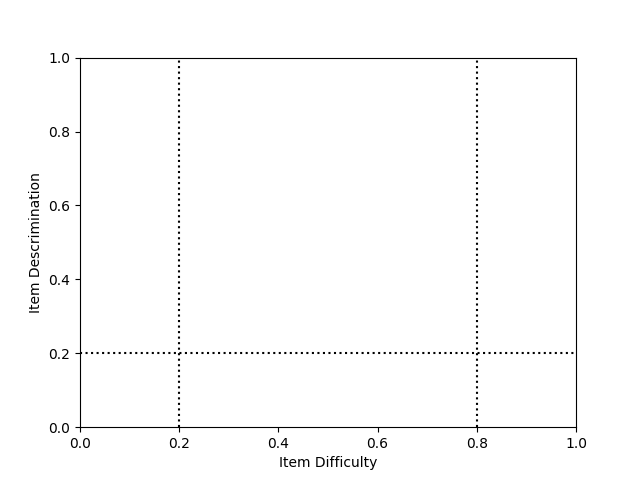
\includegraphics[scale=.5]{images/graph.png}
    \caption{Validity of Discrimination and Difficulty}
    \label{fig:ideal}
\end{center}
\end{figure}
\fi

\iflong
\section{Distractor Analysis}
\fi
\ifshort
\section{Topic Agreement and Distractor Analysis}
\fi


Distractor analysis can be used to analyze an item that's inclusion doesn't improve $\alpha$ or has a difficulty and discrimination outside the accepted range. To analyze distractors we split the students into tertiles (thirds) according to total scores. After splitting the students, take the proportion of test takers selecting each response \cite{og_ctt}. There are certain trends we expect to see. (1) The percentage of students selecting the correct answer should increase from the bottom third to the top third. (2) The item's difficulty for the top third of students should be near the upper range of accepted difficulty. (3) Each distractor is expected to have a negative discrimination value \cite{distractor}. A distractor's discrimination value is calculated by setting it as the correct answer and re-grading the student's responses. A distractor with a negative discrimination is selected more by weaker students. %If these trends do not appear the distractor may be the issue.

\section{Concept Subgroups}

Cronbach's $\alpha$ can be applied to a group of items called a \textit{subgroup}. In our case, the subgroup consists of the 5 items designed to cover the same concept. These subgroups can be evaluated separately to assess reliability to determine whether these subgroups can be tested individually. Ideally, the concept should have a reliability similar to the overall instrument. In practice, having a similar reliability to the entire instrument is difficult because each subgroup has fewer items. 


\iflong

\section{Previous Work}
\subsection{Concept Inventory Evaluation}

Because a test cannot be universally valid for every population or use, we need to carefully define the contexts, populations, and uses for which the \gls{cci} is valid. The \gls{cci} is intended to measure the cybersecurity conceptual knowledge of students who have completed a first course in cybersecurity. Cybersecurity is taught to an increasingly wide range of stakeholders, such as policy makers, computer scientists, medical professionals, and business professionals whose courses vary in focus and depth. Because of this high variance, we have chosen to optimize the \gls{cci} for the largest population of cybersecurity professionals - computer scientists. While the \gls{cci} may provide useful insights about the conceptual knowledge of policy makers or others, our goal is to have the tool provide the most insight about computer science students. 

Once an assessment tool is created, it should be administered to its targeted demographic and be statistically evaluated. \glspl{cilabel} can be powerful instruments if they actually measure students' conceptual knowledge. A minority of \glspl{cilabel} have been scrutinized using measurement or test development theories to justify being a valid and reliable research instrument \cite{dlci}. Jorian et al. \cite{jorian} outline three basic criteria of a valid \gls{cilabel}: \gls{cilabel} indicates overall understanding of the concepts, \gls{cilabel} indicates understanding of a specific concept, \gls{cilabel} indicates misconceptions or student errors.

 Jorion et al. recommend using a series of statistical tests to demonstrate whether a \gls{cilabel} meets these criteria. They recommend beginning analysis of \gls{cilabel} using \gls{ctt}. \gls{ctt} argues that an assessment tool should minimize error, possess items that all test a single construct, possess items that are neither too hard or too easy, and possess items that each provide a good estimate of a students' overall ability. 

\fi

%\glsresetall
\chapter{Methods}
The \gls{cci} has 15 scenarios, each of which describes a security problem. Each scenario of the \gls{cci} presents several question stems. Each stem is followed by five possible answer choices. One answer is correct. The other, incorrect, answers are called \textit{distractors}. Each multiple-choice question is called an \textit{item}. The current \gls{cci} has 25 items.

%\textbf{Subject: Discuss the development.}

%The CCI scenarios are based on scenarios developed by Sherman et al. \cite{scenarios}. To develop the CCI scenarios and questions, Sherman et al. held a "hackathon" with 17 experts from industry and academia. Sherman et al. collaborated with experts to develop high-quality items that are relevant to the five core security concepts. Sherman et al. performed think-aloud interviews with students about these scenarios. From the think-aloud interviews, Scheponik et al. developed common student misconceptions \cite{misconceptions}. These misconceptions were used to form the distractors of each item.

\section{Expert Panel}

We compiled the items developed and formed the \textit{initial \gls{cci}}.  The initial \gls{cci} contained 32 items. To further establish the validity of the \gls{cci}, we gave these items to an expert panel for review. The expert panel consisted of 11 professors with backgrounds in cybersecurity and 1 cybersecurity professional. These professors were from diverse universities across the country. The cybersecurity professional worked as a consultant in cybersecurity. The experts each received the initial \gls{cci} in the form of an online exam. The online exam contained each of the 32 items. Additionally, experts were asked to rank each item on the scale Accept, Accept with Minor Revisions, Accept with Major Revisions, and Reject. Included in each item, was a comment box for any written feedback from experts. Experts were instructed to leave a ranking, write any feedback, and answer the question. After answering, experts were shown the correct answer. The experts were then given the option to provide comments on the correct answer. 


To incorporate the feedback, we concluded taking expert feedback before giving it to students. The expert feedback consisted of each experts' comments and rankings. The experts' comments mainly covered issues with clarity including problems with wording and implicit assumptions. We fixed wording issues by changing the item to address the complaint and checking back with experts for approval. We also stated any assumptions that experts thought were unclear. For some items, the experts disagreed with the content or the correct answer. When the experts disagreed, we omitted that item from the \gls{cci}. After we removed these items, the experts' reviews were used to rank the remaining items. The highest ranked items were incorporated into the current \gls{cci}, demonstrating that the \gls{cci} should be validly applicable to students beyond our institutions.

\iflong

During the expert reviews, we continued developing items for the \gls{cci}. These items were intended to be used as alternates. One alternate item, Q25, was not reviewed by experts but was included. We thought this item evaluated the core concept \textit{\gls{c}} better than those that were reviewed. This item and those with the best reviews form the current 25 item \gls{cci}.

\fi


\section{Current \gls{cci}}

In attempt to meet a range of difficulties we selected items with a range of difficulties based on our best estimation. The breakdown of questions are 6 easy, 16 medium, and 3 hard. The actual performance of students will likely differ from our estimations. Each item covers one of the five major concepts shown in Table \ref{tab:topics}. \iflong The items are shown in Table \ref{tab:final_question_breakdown} in Appendix 1. This table shows the scenario, name, concept, topic of each item in the current \gls{cci}.\fi 



\glsreset{c}
\glsreset{v}
\glsreset{d}
\glsreset{g}
\glsreset{t}


\iflong
\begin{table}[!h]
\centering
\caption{Five Core Concepts of Cybersecurity}
\scalebox{.9}{
\begin{tabular}{c}
\toprule
  \gls{v}\\
  \gls{c}\\
  \gls{d}\\
  \gls{g}\\
  \gls{t}\\
\bottomrule
\end{tabular}
}
\label{tab:topics}
\end{table}
\fi
\ifshort
\begin{table}[!h]
\centering
\caption{Five Core Concepts of Cybersecurity}
\scalebox{.7}{
\begin{tabular}{c}
\toprule
  \gls{v}\\
  \gls{c}\\
  \gls{d}\\
  \gls{g}\\
  \gls{t}\\
\bottomrule
\end{tabular}
}
\label{tab:topics}
\end{table}
\fi




\FloatBarrier






\section{Pilot Trial}

The goal of the pilot trial was to administer the current \gls{cci} to a small group of 100-200 students. Then use the results of this pilot trial to suggest modifications to the assessment. The pilot trial was completed in December, 2018 by 142 students from 6 universities.

Professors at each university had the option of administering a paper version or online version of the \gls{cci}. Both versions included instructions at the beginning of the exam. \iflong The instructions can be seen in Appendix 2. \fi Both versions also had all of the items belonging to the same scenario appear sequentially. The distractors, scenarios, and questions were identical in both versions. 

If the professors decided to administer the paper version, the professor proctored this version as an exam. To proctor the exam, a professor allocated 50 minutes for students to take the exam in class. Students then completed the exam to the best of their abilities. The professor collected the exam papers and sent them to us. We then recorded each student's response to every item. 

If the professor decided to administer the online version, students were provided a link to the exam. The online exam differed from the paper version in three ways. First, the online version had a random ordering of distractors. Second, items that shared a scenario were randomly ordered within that scenario. For example, if Q1 and Q2 are the two items in the one scenario, Q1 can appear before or after Q2. However, they would always appear together. Third, there was no hard time limit. Students were told to spend 50 minutes but this was not strictly enforced. The student completed the exam and then selected a submit button. After selecting submit, the students responses were saved.


\FloatBarrier
\section{Pilot Demographics}

The universities included in the pilot trial have diverse locations and populations. Universities A and D are large Midwestern public universities and have over 40 thousand students enrolled. University E is a large public university from the South with over 40 thousand students enrolled. University B, C, F are smaller universities from the Midwestern and Eastern part of the country. These Universities have 10k or less students enrolled.

The demographics of the study including institution and response rate are in Table \ref{tab:student_breakdown}. University A was the only group given the assessment in paper format. The professors at the other Universities sent out the link to the assessment to the students in the course. With one exception, at University D the assessment was to the 6 member of this club who are taking this course. This club sent out the link to members who were taking the first cybersecurity course. 



\iffalse
\begin{table}[!htbp]
\centering
\begin{tabular}{cc}
    \toprule
    \textbf{University/Organization} & \textbf{Number of Experts}\\
    \midrule
    \textit{University of Utah} & 1\\
    \textit{Capitol Tech} & 1\\
    \textit{Texas A \& M} & 1\\
    \textit{University of Southern California} & 1\\
    \textit{Association for Computing Machinery (ACM)} & 1\\
    \textit{University A} & 2\\
    \textit{Depaul University} & 1\\
    \textit{Michigan Tech University} & 1\\
    \textit{University G} & 1\\
    \textit{Montgomery College} & 1\\
    \textit{University B} & 1\\
    \textif{No University Specfified} & 4\\
    \midrule
    \textit{Total} & 12\\
    \bottomrule
\end{tabular}   
\caption{Breakdown of Professors By University/Organization}
\label{tab:proffesor_breakdown}
\end{table}
\fi

\iflong
\begin{table}[!htbp]
\caption{Breakdown of Students by University}
\centering
\scalebox{.6}{
\begin{tabular}{cS[table-number-alignment = center]S[table-number-alignment = center]S[table-number-alignment = center]}
    \toprule
    \textbf{University} & \textbf{Number of Students} & \textbf{Potential Number of Students} & \textbf{Response Rate (\%)}\\
    \midrule
    \textit{University A} & 91 & 120 & 76 \\
    \textit{University B} & 12 & 20 & 60 \\
    \textit{University C} & 1 & 12 & 16\\
    \textit{University D} & 6 & 6 & 100 \\   
    \textit{University E} & 17 & 50 & 34 \\
    %\textit{University F} & 6 & 40 & 15 \\
    \textit{University F} &	12 & 20 & 60\\
    \textit{No University Specified} & 3 &  & \\
    \midrule
    \textit{Total} & 142 & 228 & 62 \\
    \bottomrule
\end{tabular}   
}

\label{tab:student_breakdown}
\end{table}
\fi

\ifshort
\begin{table}[!htbp]
\centering
\scalebox{.6}{
\begin{tabular}{cc}
    \toprule
    \textbf{University} & \textbf{Number of Students}\\
    \midrule
    \textit{University A} & 91  \\
    \textit{University B} & 14  \\
    \textit{University C} & 1 \\
    \textit{University D} & 6  \\   
    \textit{University E} & 17 \\
    %\textit{University F} & 6 & 40 & 15 \\
    \textit{University F} &	12\\
    \textit{No University Specified} & 3 \\
    \midrule
    \textit{Total Number of Completed Exams} & 142\\
    \bottomrule
\end{tabular}   
}
\caption{Breakdown of Students By University}
\label{tab:student_breakdown}
\end{table}
\fi

\iffalse
\begin{table}[!htbp]
\centering
\begin{tabular}{cc}
    \toprule
    \textbf{Year} & \textbf{Number of Students}\\
    \midrule
    \textit{Sophomore} & 79 \\
    \textit{Junior} & 24 \\
    \textit{Senior} & 29 \\
    \textit{Graduate} & 11 \\   
    \bottomrule
\end{tabular}   
\caption{Breakdown of Students By Year}
\label{tab:student_year}
\end{table}
\fi

%\glsresetall
\chapter{Results}
%\textbf{Subject: Results contain expert panel and pilot study.}

%The intention of this \DocTitle  is to evaluate the current \gls{cci}. The evaluation of the \gls{cci} involved two stages, expert panel review and pilot testing with students. The expert panel was given to 12 experts each from a different institution. The experts provided comments and reviews to improve the final instrument. After the expert panel, the pilot instrument was taken by 142 students from 6 institutions. By using multiple institutions, the study encompasses a good sample that covers different courses and teaching styles.

In this section, we present results from the expert review of the \gls{cci} and our psychometric analysis of students' responses to the \gls{cci}. To help the reader interpret our findings, we compare our results with three \glspl{cilabel} evaluated with the same techniques. These \glspl{cilabel} are the Concept Assessment Tool for Statics (27 questions and 1,372 students), the Statistics Concept Inventory (38 questions and 402 students), and the Dynamics Concept Inventory (29 questions and 5,966 students) \cite{jorian}. We chose these \glspl{cilabel} because they are the few technical \glspl{cilabel} that have been analyzed using similar techniques.


%\textbf{Subject: Describe what the goal of the results.}

%To evaluate the pilot study we used conventional psychometrics associated with \gls{ctt}. These techniques include difficulty and discrimination to assess the quality of individual items. Cronbach's $\alpha$ to assess both the reliability of the instrument and the quality of specific items. \iflong \gls{efa} to evaluate the correlation of items in the same concepts. \fi 



\section{Expert Panel}

The expert panel consisted of 12 experts in cybersecurity or a related field. These experts reviewed each of the individual items and rated them on a scale of Accept, Accept with Minor Revisions, Accept with Major Revisions, and Reject. The results of this review process can be seen in Figure \ref{fig:accept_rej}. This figure includes the items in the current assessment although a total of 32 items were reviewed. The items selected for the \gls{cci} were reviewed positively receiving a vast majority of Accept and Accept with Minor Revisions. Of the questions that received rejects, they received helpful comments to address the source of the rejection. These results provide evidence for the validity of the chosen items in the \gls{cci}.

\iflong
\begin{figure}[!htbp]
    \begin{center}
    \advance\leftskip-3cm
    \advance\rightskip-3cm
    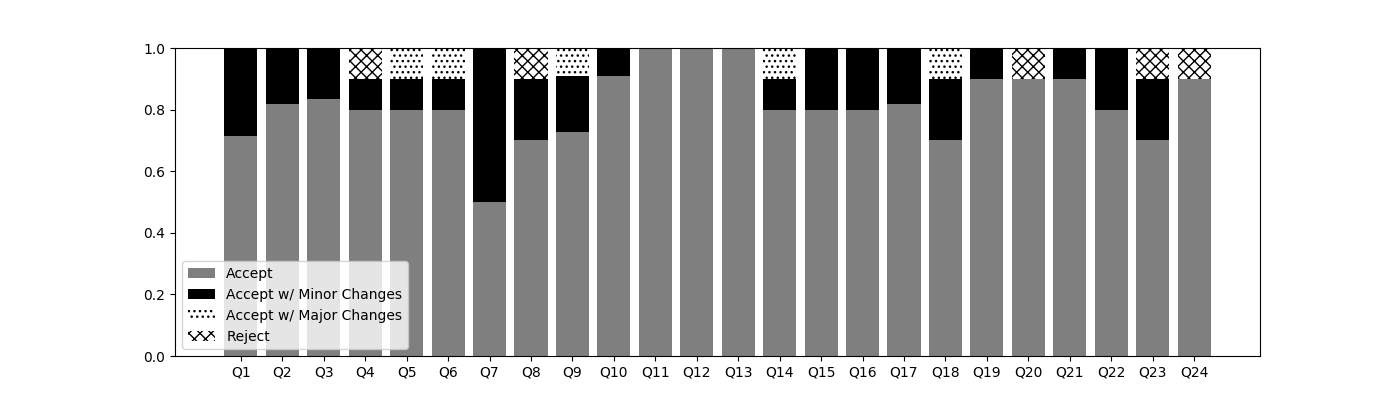
\includegraphics[scale=.5]{images/bar.png}
    \caption{Expert Response to Items}
    \label{fig:accept_rej}
\end{center}
\end{figure}
\fi

\ifshort
\begin{figure}[!htbp]
    \begin{center}
    \advance\leftskip-3cm
    \advance\rightskip-3cm
    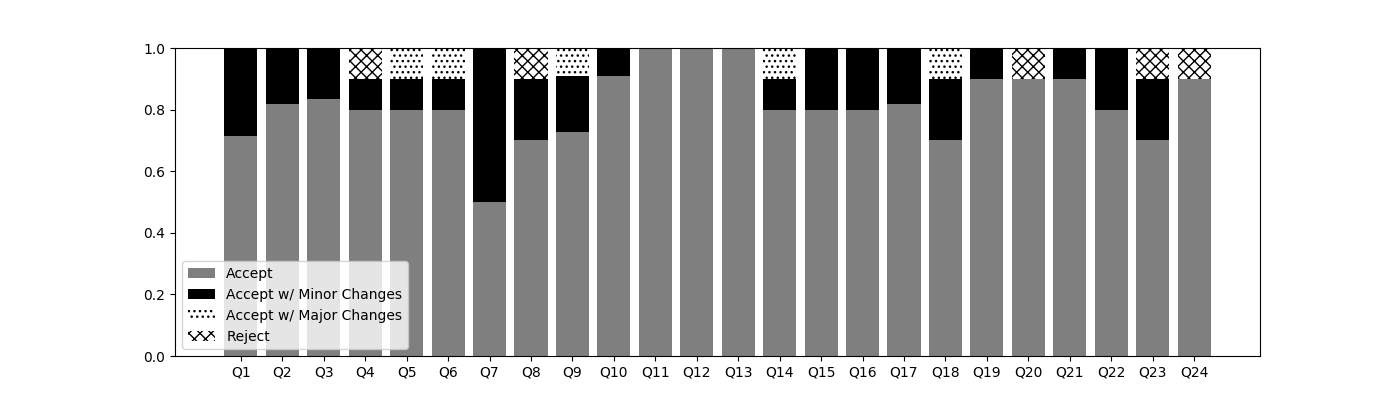
\includegraphics[scale=.3]{images/bar.png}
    \caption{Expert Response to Items}
    \label{fig:accept_rej}
\end{center}
\end{figure}
\fi

\FloatBarrier
\section{Reliability and Standard Error}

Cronbach's $\alpha$ is a measure of the reliability of the instrument. Jorian et al. \cite{jorian} describes anything above 0.8 as good and Panayiotis \cite{panayiotis} describes 0.7 as the minimum. The reliability of the \gls{cci} in this pilot test is 0.78 which is close to Jorian et al's recommendation for good reliability and above Panayiotis's minimum recommendation. The reliability of the \gls{cci} is strong when compared to other \glspl{cilabel}. The Concept Assessment Tool for Statics, the Statistics Concept Inventory, and the Dynamics Concept Inventory had $\alpha$ values of 0.84, 0.64, and 0.74 respectively \cite{jorian}. The reliability of the \gls{cci} suggests that it is sufficiently reliable to be a valid \gls{cilabel}.

The standard error of measurement defines a confidence interval for each student's true score. The standard measurement error of the \gls{cci} was 2.13 for this pilot test. A 2.13 standard error implies the 68\% confidence interval for a student’s true score, given a mean observed score of 9 points (approximating mean of 8.610), is from 6.87 to 11.13. Given this interval, students with total scores anywhere between 7 and 11 have a 68\% confidence that students have different true scores. 

%The Concept Assessment Tool for Statics, the Statistics Concept Inventory, and the Dynamics Concept Inventory had standard error of measurement values of 2.02, 2.21, 2.02 respectively \cite{jorian}. The \gls{cci} performs well compared to these studies, which is expected given the $\alpha$ values.

\begin{table}[!htbp]
\caption{Instrument Statistics}
\centering
\begin{tabular}{cc}
    \toprule
    \textit{Cronbach's $\alpha$} & 0.78 \\
    \textit{Standard Error of Measurement} & 2.13 \\
    \textit{Mean (Out of 25)} & 8.61\\
    \textit{Standard Deviation} & 4.58\\
    \bottomrule
\end{tabular}
\label{tab:overall}
\end{table}


Cronbach's $\alpha$ can be used as a coarse evaluation of the quality of an item. Each item should increase the quality of the instrument and excluding that item should decrease the overall reliability. Table \ref{tab:table_cronbach_exclusion} shows the results of the Cronbach calculation with each item excluded. Ideally, every item would be below the original Cronbach $\alpha$ indicating that each item increases the overall reliability. There are no items that decrease the overall reliability and consequently need to be removed.

\iffalse
\iflong
\begin{figure}[ht]
    \begin{center}
    \advance\leftskip-.25cm
    \advance\rightskip-.25cm
    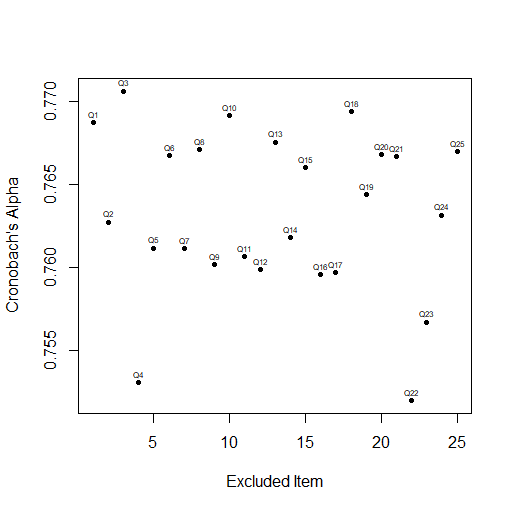
\includegraphics[scale=.5]{images/Cronobach's.png}
    \caption{Cronbach's $\alpha$ with Items Excluded}
    \label{fig:cron}
\end{center}
\end{figure}
\fi
\fi

\begin{table}[!htbp]
%\begin{subtable}[t]{0.45\textwidth}
%\begin{tabular}[t]{@{} l c *{5}{d{1.7}} @{}}
\caption{Cronbach's $\alpha$ Analysis}
\begin{subtable}[!htbp]{0.45\textwidth}
\flushright
%\begin{tabular}[t]{@{} l c *{2}{d{2}} @{}}
\begin{tabular}[!htbp]{c c}
\toprule
Item Excluded & Cronbach's $\alpha$ \\
\textit{Q1} & 0.77 \\
\textit{Q2} & 0.76 \\
\textit{Q3} & 0.78 \\
\textit{Q4} & 0.76 \\
\textit{Q5} & 0.76 \\
%\bottomrule
\end{tabular}
%\caption{\footnotesize Question 3 Distractors}
\label{tab:table2_a}
\end{subtable}
\hspace{\fill}
\begin{subtable}[!htbp]{0.45\textwidth}
\flushright
%\begin{tabular}[t]{@{} l c *{2}{d{2}} @{}}
\begin{tabular}[!htbp]{c c}
\toprule
Item Excluded & Cronbach's $\alpha$ \\
\textit{Q6} & 0.77 \\
\textit{Q7} & 0.77 \\
\textit{Q8} & 0.77 \\
\textit{Q9} & 0.76 \\
\textit{Q10} & 0.77 \\
%\bottomrule
\end{tabular}
%\caption{\footnotesize Question 3 Distractors}
\label{tab:table2_b}
\end{subtable}
\hspace{\fill}
\begin{subtable}[!htbp]{0.45\textwidth}
\flushright
%\begin{tabular}[t]{@{} l c *{2}{d{2}} @{}}
\begin{tabular}[!htbp]{c c}
\toprule
Item Excluded & Cronbach's $\alpha$ \\
\textit{Q11} & 0.76 \\
\textit{Q12} & 0.76 \\
\textit{Q13} & 0.77 \\
\textit{Q14} & 0.76 \\
\textit{Q15} & 0.77 \\
\bottomrule
\end{tabular}
%\caption{\footnotesize Question 3 Distractors}
\label{tab:table2_c}
\end{subtable}
\hspace{\fill}
\begin{subtable}[!htbp]{0.45\textwidth}
\flushright
%\begin{tabular}[t]{@{} l c *{2}{d{2}} @{}}
\begin{tabular}[!htbp]{c c}
\toprule
Item Excluded & Cronbach's $\alpha$ \\
\textit{Q16} & 0.76 \\
\textit{Q17} & 0.76 \\
\textit{Q18} & 0.77 \\
\textit{Q19} & 0.77 \\
\textit{Q20} & 0.77 \\
\bottomrule
\end{tabular}
%\caption{\footnotesize Question 3 Distractors}
\label{tab:table2_d}
\end{subtable}
\hspace{\fill}
\begin{subtable}[!htbp]{\textwidth}
\center
%\begin{tabular}[t]{@{} l c *{2}{d{2}} @{}}
\begin{tabular}[!htbp]{c c}
\\
\toprule
Item Excluded & Cronbach's $\alpha$ \\
\textit{Q21} & 0.77 \\
\textit{Q22} & 0.76 \\
\textit{Q23} & 0.76 \\
\textit{Q24} & 0.77 \\
\textit{Q25} & 0.77 \\
\bottomrule
\end{tabular}
%\caption{\footnotesize Question 3 Distractors}
\label{tab:table2_e}
\end{subtable}
\hspace{\fill}
\label{tab:table_cronbach_exclusion}
\end{table}



\FloatBarrier
\section{Difficulty and Discrimination}

Difficulty is the fraction of students with the correct response. If an item is too hard, the item is separating only strong students from strong students. If an item is too easy, it cannot differentiate any students. The acceptable range of difficulty is between 0.2 and 0.8 percent. The difficulty of each item can be seen in Figure \ref{fig:dif_disc} and Table \ref{tab:diff_v_discrimination}. The range of difficulty is 0.1 to 0.66. The Concept Assessment Tool for Statics, the Statistics Concept Inventory, and the Dynamics Concept Inventory had difficulty ranges of 0.16 to 0.78, 0.03 to 0.87 and 0.06 to 0.91 respectively. The instrument overall is too difficult as evident by 21 out of 25 items having difficulty below 0.5 and 5 items falling outside the minimum acceptable difficulty. 

The discrimination indicates the amount of information an item gives about the overall performance of the student. High discrimination indicates that a student performance on a given item is highly correlated to overall performance. The acceptable range of discrimination is anything above 0.2. Discrimination can be seen in Figure \ref{fig:dif_disc}. The range of discrimination if 0.16 to 0.47. The Concept Assessment Tool for Statics, the Statistics Concept Inventory, and the Dynamics Concept Inventory had discrimination ranges of 0.18 to 0.65, -0.13 to 0.57 and 0.01 to 0.56 respectively. Those \glspl{cilabel} had 1, 10, and 5 items fall below the 0.2 minimum values compared to the \gls{cci} with 3 items that fall below 0.2. The discrimination range is not as high as other \glspl{cilabel}, but the bottom of the range is good when compared to other \glspl{cilabel}.

\iffalse
\iflong
The correlation coefficient can be calculated for each item to quantify how similar the item fits in with the rest of the items. The correlation for each item can be seen in Figure \ref{fig:correlation}. 


\begin{figure}[!hbp]
    \begin{center}
    \advance\leftskip-3cm
    \advance\rightskip-3cm
    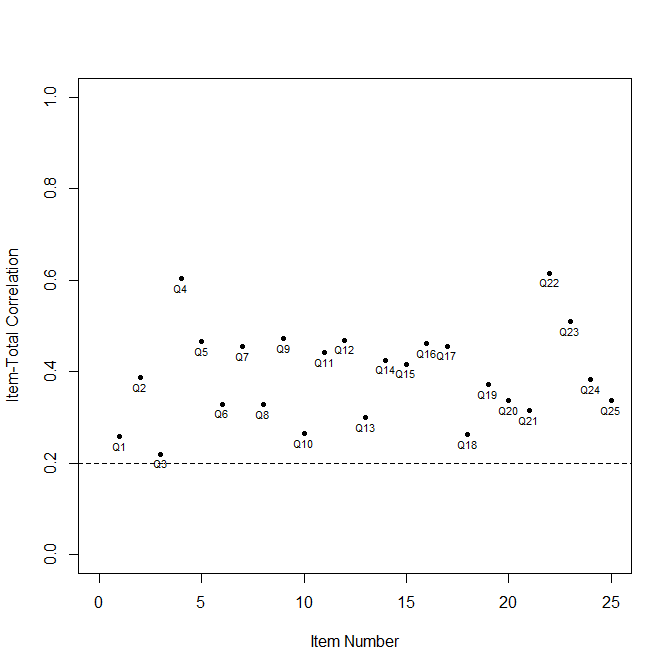
\includegraphics[scale=.45]{images/correlation.png}
    \caption{Correlation}
    \label{fig:correlation}
\end{center}
\end{figure}
\fi
\fi

\begin{table}[!htbp]
\caption{Difficulty and Discrimination of Each Item}
\centering
\scalebox{.7}{
\begin{tabular}{cccccc}
    \toprule
    Item & Discrimination & Difficulty & Item & Discrimination & Difficulty\\
    \midrule
    \textit{Q1} & 0.22 & 0.24 & \textit{Q14} & 0.32 & 0.25 \\
    \textit{Q2} & 0.32 & 0.33 & \textit{Q15} & 0.25 & 0.10 \\
    \textit{Q3} & 0.16 & 0.26 & \textit{Q16} & 0.35 & 0.59 \\
    \textit{Q4} & 0.46 & 0.52 & \textit{Q17} & 0.35 & 0.52 \\
    \textit{Q5} & 0.35 & 0.18 & \textit{Q18} & 0.19 & 0.31 \\
    \textit{Q6} & 0.23 & 0.22 & \textit{Q19} & 0.27 & 0.28 \\
    \textit{Q7} & 0.30 & 0.66 & \textit{Q20} & 0.22 & 0.14 \\
    \textit{Q8} & 0.21 & 0.19 & \textit{Q21} & 0.23 & 0.44 \\
    \textit{Q9} & 0.33 & 0.61 & \textit{Q22} & 0.47 & 0.34 \\
    \textit{Q10} & 0.19 & 0.4 & \textit{Q23} & 0.38 & 0.49 \\
    \textit{Q11} & 0.34 & 0.36 & \textit{Q24} & 0.30 & 0.40 \\
    \textit{Q12} & 0.36 & 0.24 & \textit{Q25} & 0.24 & 0.14 \\
    \textit{Q13} & 0.21 & 0.28 & \textit{} &  &\\
    \bottomrule
\end{tabular}
}
\label{tab:diff_v_discrimination}
\end{table}




\begin{figure}[ht]
    \begin{center}
    \advance\leftskip-.25cm
    \advance\rightskip-.25cm
    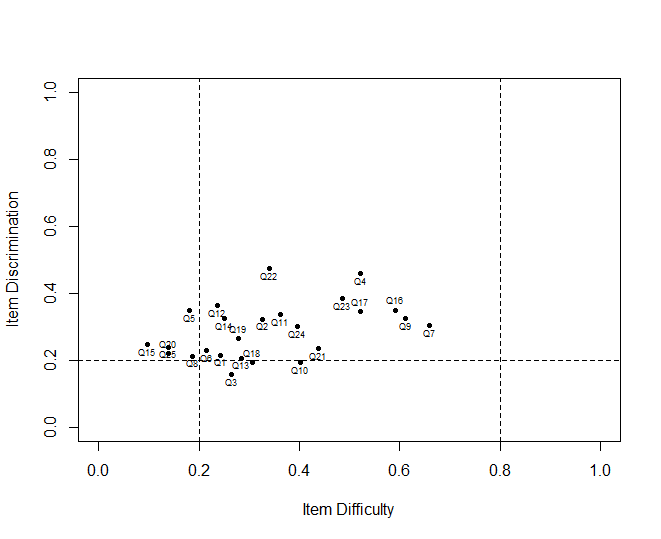
\includegraphics[scale=.45]{images/diff_v_discrimination_full.png}
    \caption{Difficulty vs. Discrimination}
    \label{fig:dif_disc}
\end{center}
\end{figure}



\FloatBarrier
\section{Concept Subtests}
The \gls{cci} consists of five concepts: \gls{v}, \gls{c}, \gls{d}, \gls{g}, and \gls{t}. Each item assesses one of these concepts. The individual items within a concept can be grouped and the Cronbach's $\alpha$ calculated to evaluate the reliability of that concept subtest. The $\alpha$'s of the concept subtests are seen in Table \ref{tab:alpha_concept}. When evaluating the concepts, it is notable that all of the values are significantly less than 0.7 which is considered the minimal acceptable value for a reliable assessment \cite{panayiotis}. These findings suggest that it is not recommended to use the subtests as evaluations of students' knowledge of the specific concepts. 

%Specifically, \gls{v} has a poor $\alpha$ of 0.236 indicating that the evaluation of that concept through this \gls{cci} is not practical. 

\begin{table}[!htbp]
\caption{Cronbach's $\alpha$ by Concept}
\centering
\scalebox{.8}{
\begin{tabular}{ccc}
    \toprule
    Concept & Cronbach's $\alpha$ & Items Included \\
    \midrule
    \textit{V} & 0.22 & Q1, Q3, Q11, Q17, Q21\\
    \textit{C} & 0.45 & Q2, Q5, Q14, Q18, Q24\\
    \textit{D} & 0.47 & Q4, Q6, Q13, Q19, Q23\\
    \textit{G} & 0.36 & Q8, Q9, Q10, Q22, Q25\\
    \textit{T} & 0.50 & Q7, Q12, Q15, Q16, Q20\\
    \bottomrule
\end{tabular}
}
\label{tab:alpha_concept}
\end{table}


\iflong

The correlation between items in the subtests can be expressed with a correlation matrix. The correlation matrix is the correlation coefficient of each item with every other item. A heat map of the correlation matrix can be seen in Figure \ref{fig:alignment}. The square regions are all items in a specific concept subtest. Items within the same concept subtest should be expected to have  greater correlation  with each other than with items outside their subtest. We do not see this type of stronger and weaker correlations, confirming that the concept subtests cannot be used as standalone assessments.

\begin{figure}[!hbp]
    \centering
    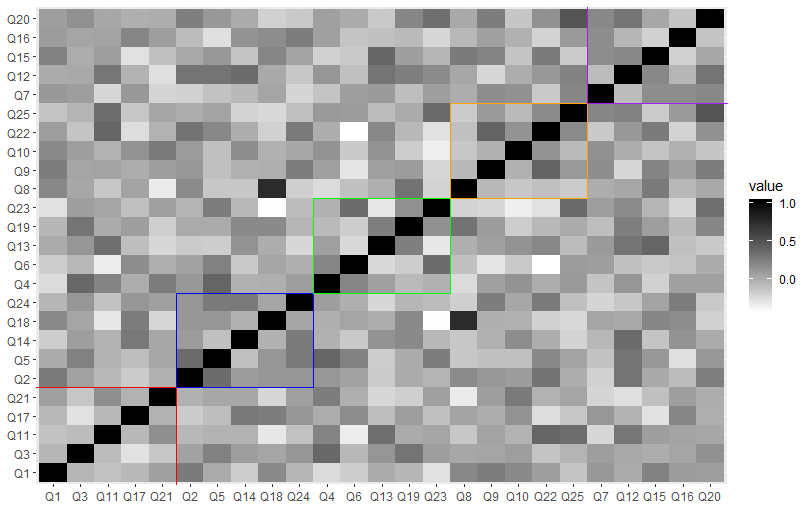
\includegraphics[scale=.35]{images/heat_map_top_quarter.png}
    \begin{minipage}{0.65\linewidth}
    \tiny
    \emph{
    V: Red,
    C: Blue,
    D: Green,
    G: Orange,
    T: Purple
    }
    \end{minipage}
    \caption{Concept Alignment of Top Quarile}
    \label{fig:alignment}
\end{figure}
\fi

\iffalse
%Remove \gls{efa}. If there is strong evidence from \gls{ctt} that it is a unidimensional test there is no need for an \gls{efa}.
%\gls{efa} is a factor analysis that attempts to determine whether the multiple domain concepts are related. We used oblique rotation which assumes an underlying assumption that the factors are correlated. Rather than use it as a heuristic we used five factors because this is the number of concepts designed. This analysis seen in Table \ref{tab:efa}. The ideal result would be clear factors that divide the questions into the corresponding concepts. The squares attempt to cluster the factors by the concepts. However, this is not possible  the items within the same concept not sharing obvious factors. 


%\begin{table}[!htbp]
%\caption{Exploratory Factor Analysis}
%\centering
%\scalebox{.8}{
%\begin{tabular}{llllll}
%\toprule
%Item & V & G & T & C & D \\
%\midrule
%\\\cline{2-2}
%\textit{Q1} & \multicolumn{1}{|c|}{0.29} &  &  &  &  \\
%\textit{Q3} & \multicolumn{1}{|c|}{} &  & 0.31 &  &  \\
%\textit{Q11} & \multicolumn{1}{|c|}{0.55} &  &  &  &  \\
%\textit{Q17} & \multicolumn{1}{|c|}{} & 0.28 &  &  &  \\
%\textit{Q21} & \multicolumn{1}{|c|}{0.21} &  &  &  &  \\\cline{2-2}  \cline{3-3}
%\textit{Q8} &  & \multicolumn{1}{|c|}{0.56} &  &  &  \\
%\textit{Q9} &  & \multicolumn{1}{|c|}{0.24} &  &  &  \\
%\textit{Q10} & 0.36 & \multicolumn{1}{|c|}{}  &  &  &  \\
%\textit{Q22} & 0.55 & \multicolumn{1}{|c|}{}  &  &  &  \\
%\textit{Q25} &  & \multicolumn{1}{|c|}{}  & 0.55 &  &  \\\cline{3-3}\cline{4-4}
%\textit{Q7} &  & 0.3 & \multicolumn{1}{|c|}{} &  &  \\
%\textit{Q12} &  & & \multicolumn{1}{|c|}{0.47} &  &  \\
%\textit{Q15} &  & 0.25 & \multicolumn{1}{|c|}{} &  &  \\
%\textit{Q16} &  &  & \multicolumn{1}{|c|}{} &  & 0.54 \\
%\textit{Q20} &  &  & \multicolumn{1}{|c|}{0.58} &  &  \\\cline{4-4}\cline{5-5}
%\textit{Q2} &  &  &  & \multicolumn{1}{|c|}{0.36} &  \\
%\textit{Q5} &  &  &  & \multicolumn{1}{|c|}{0.5} &  \\
%\textit{Q14} &  &  &  & \multicolumn{1}{|c|}{0.24} &  \\
%\textit{Q18} &  & 0.6 &  & \multicolumn{1}{|c|}{} &  \\
%\textit{Q24} & &  &  & \multicolumn{1}{|c|}{0.23} &  \\\cline{5-5} \cline{6-6}
%\textit{Q4} & 0.3 &  &  &  & \multicolumn{1}{|c|}{} \\
%\textit{Q6} &  &  &  & 0.57 & \multicolumn{1}{|c|}{} \\
%\textit{Q13} & 0.49 &  &  &  & \multicolumn{1}{|c|}{} \\
%\textit{Q19} & 0.22 &  &  &  & \multicolumn{1}{|c|}{} \\
%\textit{Q23} & &  &  & 0.37 & \multicolumn{1}{|c|}{} \\\cline{6-6}
%\bottomrule
%\end{tabular}
%}
%
%\label{tab:efa}
%\end{table}

\fi



\FloatBarrier
\section{Deeper Analysis of Specific Items}

The psychometric analysis of the \gls{cci} revealed that the assessment has too many difficult items. To inform future revisions of the \gls{cci}, we are analyzing the distractor distribution and distractor discrimination to understand why some items are so difficult. We present an example of this for one of these items Q15. Q15 had a low difficulty of 0.10 and a relatively low discrimination of 0.25 in the pilot trial. We compare Q15 to a stronger item Q4 which had a good difficulty of 0.52 and a discrimination of 0.46 in the pilot trial. 

The distractor analysis shows the proportion of the students' responses in each tertile. The distractor analysis for both Q15 and Q4 can be seen in Table \ref{tab:table_distract}. In Q4, which has a good distribution, the percentage of students getting the correct answer increases from the bottom tertile to the top and the top tertile generally answers the question correct. For Q15, although, the percentage of students selecting the correct answer increases from the bottom tertile to the top, there is little difference between the top and middle tertile. Additionally, the top tertile students only get the correct answer 18\% of the time and instead select distractor A 59\% of the time. The preference for option A among the top tertile is causing the item to be too difficult.

\begin{table}[!htbp]
\caption{Distractor Distribution}
\hspace{\fill}
\begin{subtable}[!htbp]{0.45\textwidth}
\flushright
\scalebox{.9}{
\begin{tabular}[!htbp]{c c c c}
\toprule
\textbf{Q4} &  &  &  \\
\midrule
\textit{Response} & \textit{Lower} & \textit{Middle} & \textit{Upper} \\
A & 0.02 & 0 & 0.03 \\
*B & 0.28 & 0.62 & 0.85 \\
C & 0.11 & 0 & 0.26 \\
D & 0.37 & 0.14 & 0 \\
E & .22 & 0.24 & 0.10 \\
blank & 0.02 & 0 & 0 \\
\bottomrule
\end{tabular}
}
\label{tab:table1_d}
\end{subtable}
\hspace{\fill}
\begin{subtable}[!htbp]{0.45\textwidth}
\flushright
\scalebox{.9}{
\begin{tabular}[!htbp]{c c c c}
\toprule
\textbf{Q15} &  &  &  \\
\midrule
\textit{Response} & \textit{Lower} & \textit{Middle} & \textit{Upper} \\
A & 0.22 & 0.36 & 0.59 \\
B & 0.39 & 0.26 & 0.08 \\
C & 0.15 & 0.17 & 0.15 \\
D & 0.22 & 0.05 & 0 \\
*E & 0 & 0.17 & 0.18 \\
blank & 0.02 & 0 & 0 \\
\bottomrule
\end{tabular}
}
\label{tab:table1_d}
\end{subtable}
\label{tab:table_distract}
\end{table}



\iffalse
\hspace{\fill}
\begin{subtable}[!htbp]{0.45\textwidth}
\flushright
\scalebox{.9}{
\begin{tabular}[!htbp]{c c c c}
\toprule
\textbf{Q22} &  &  &  \\
\midrule
\textit{Response} & \textit{Lower} & \textit{Middle} & \textit{Upper} \\
A & 0.06 & 0.02 & 0\\
B & 0.13 & 0.071 & 0.02\\
blank & 0.04 & 0 & 0\\
C & 0.50 & 0.60 & 0.23\\
*D & 0.15 & 0.29 & 0.74\\
E & 0.13 & 0.02 & 0\\
\bottomrule
\end{tabular}
}
\label{tab:table1_d}
\end{subtable}


\begin{subtable}[!htbp]{0.5\textwidth}
\flushright
\scalebox{.9}{
\begin{tabular}[!htbp]{c c c c}
\toprule
\textbf{Q3} &  &  &   \\
\midrule
\textit{Response} & \textit{Lower} & \textit{Middle} & \textit{Upper} \\
A & 0.37 & 0.429 & 0.256 \\
B & 0.13 & 0.238 & 0.128 \\
C & 0.204 & 0.024 & 0.103 \\
*D & 0.204 & 0.214 & 0.436 \\
E & 0.093 & 0.095 & 0.077 \\
blank & 0 & 0 & 0 \\
\bottomrule
\end{tabular}
}
%\caption{\footnotesize Question 3 Distractors}
\label{tab:table1_a}
\end{subtable}
\begin{table}[!htbp]
\caption{Distractor Distribution}
\begin{subtable}[!htbp]{0.5\textwidth}
\flushright
\scalebox{.66}{
\begin{tabular}[!htbp]{c c c c}
\toprule
\textbf{Q3} &  &  &   \\
\midrule
\textit{Response} & \textit{Lower} & \textit{Middle} & \textit{Upper} \\
A & 0.37 & 0.429 & 0.256 \\
B & 0.13 & 0.238 & 0.128 \\
C & 0.204 & 0.024 & 0.103 \\
*D & 0.204 & 0.214 & 0.436 \\
E & 0.093 & 0.095 & 0.077 \\
blank & 0 & 0 & 0 \\
\bottomrule
\end{tabular}
}
%\caption{\footnotesize Question 3 Distractors}
\label{tab:table1_a}
\end{subtable}
\hspace{\fill}
\begin{subtable}[!htbp]{0.5\textwidth}
\flushright
\scalebox{.66}{
\begin{tabular}[!htbp]{c c c c}
\toprule
\textbf{Q5} &  &  &   \\
\midrule
\textit{Response} & \textit{Lower} & \textit{Middle} & \textit{Upper} \\
A & 0.389 & 0.524 & 0.308 \\
B & 0.167 & 0.071 & 0.051 \\
C & 0.278 & 0.167 & 0.128 \\
D & 0.074 & 0.167 & 0.077 \\
*E & 0.093 & 0.071 & 0.436 \\
blank & 0 & 0 & 0 \\
\bottomrule
\end{tabular}
}
\label{tab:table1_b}
\end{subtable}
\hspace{\fill}
\begin{subtable}[!htbp]{0.5\textwidth}
\flushright
\scalebox{.66}{
\begin{tabular}[!htbp]{c c c c}
\toprule
\textbf{Q8} &  &  &  \\
\midrule
\textit{Response} & \textit{Lower} & \textit{Middle} & \textit{Upper} \\
A & 0.333 & 0.357 & 0.154 \\
B & 0.463 & 0.31 & 0.513 \\
*C & 0.074 & 0.238 & 0.333 \\
D & 0.074 & 0 & 0 \\
E & 0.056 & 0.095 & 0 \\
blank & 0 & 0 & 0 \\
\bottomrule
\end{tabular}
}
\label{tab:table1_c}
\end{subtable}
\hspace{\fill}
\begin{subtable}[!htbp]{0.5\textwidth}
\flushright
\scalebox{.66}{
\begin{tabular}[!htbp]{c c c c}
\toprule
\textbf{Q15} &  &  &  \\
\midrule
\textit{Response} & \textit{Lower} & \textit{Middle} & \textit{Upper} \\
A & 0.222 & 0.357 & 0.59 \\
B & 0.389 & 0.262 & 0.077 \\
C & 0.148 & 0.167 & 0.154 \\
D & 0.222 & 0.048 & 0 \\
*E & 0 & 0.167 & 0.179 \\
blank & 0.019 & 0 & 0 \\
\bottomrule
\end{tabular}
}
\label{tab:table1_d}
\end{subtable}
\hspace{\fill}
\begin{subtable}[!htbp]{0.5\textwidth}
\flushright
\scalebox{.66}{
\begin{tabular}[!htbp]{c c c c}
\toprule
\textbf{Q20} &  &  &  \\
\midrule
\textit{Response} & \textit{Lower} & \textit{Middle} & \textit{Upper} \\
A & 0.222 & 0.143 & 0 \\
*B & 0.074 & 0.167 & 0.231 \\
C & 0.333 & 0.262 & 0.308 \\
D & 0.222 & 0.119 & 0.051 \\
E & 0.093 & 0.31 & 0.41 \\
blank & 0.056 & 0 & 0 \\
\bottomrule
\end{tabular}
}
\label{tab:table1_e}
\end{subtable}
\hspace{\fill}
\begin{subtable}[!htbp]{0.5\textwidth}
\flushright
\scalebox{.66}{
\begin{tabular}[!htbp]{c c c c}
\toprule
\textbf{Q25} &  &  &  \\
\midrule
\textit{Response} & \textit{Lower} & \textit{Middle} & \textit{Upper} \\
*A & 0.093 & 0.095 & 0.282 \\
B & 0.241 & 0.286 & 0.205 \\
C & 0.259 & 0.19 & 0.128 \\
D & 0.167 & 0.167 & 0.128 \\
E & 0.204 & 0.262 & 0.256 \\
blank & 0.037 & 0 & 0 \\
\bottomrule
\end{tabular}
}
\label{tab:table1_f}
\end{subtable}
\label{tab:table_distract}
\end{table}
\fi

\FloatBarrier
 
 Table \ref{tab:table_distract_discrim} shows the discrimination of each distractor for both Q4 and Q15. We expect the distractors to have negative discrimination values. Q4 has negative or zero values for each distractor as well as a large positive discrimination for the correct answer. Q15 does have a large positive discrimination for the correct answer and is even above the minimum acceptable value, but distractor A has a larger, positive discrimination value. This analysis reveals that for some reason the correct answer is not compelling to the strongest students, suggesting that the wording or structure of the answer choices may be to blame. We explore this assertion more in the future work.

\begin{table}[!htbp]
\caption{Distractor Discrimination}
\hspace{\fill}
\begin{subtable}[!htbp]{0.45\textwidth}
\flushright
\scalebox{1}{
\begin{tabular}[!htbp]{c c}
\toprule
\textbf{Q4} &  \\
\midrule
\textit{Distractor} & \textit{Discrimination} \\
A & 0 \\
*B & 0.46 \\
C & -0.14 \\
D & -0.26 \\
E & -0.04 \\
\bottomrule
\end{tabular}
}
\label{tab:table4_c}
\end{subtable}
\hspace{\fill}
\begin{subtable}[!htbp]{0.45\textwidth}
\flushright
\scalebox{1}{
\begin{tabular}[!htbp]{c c}
\toprule
\textbf{Q15} & \\
\midrule
\textit{Distractor} & \textit{Discrimination} \\
A & 0.35  \\
B & -0.19 \\
C & 0 \\
D & -0.26 \\
*E & 0.24  \\
\bottomrule
\end{tabular}
}
\label{tab:table4_d}
\end{subtable}
\label{tab:table_distract_discrim}
\end{table}



\iffalse

\hspace{\fill}
\begin{subtable}[!htbp]{0.45\textwidth}
\flushright
\scalebox{1}{
\begin{tabular}[!htbp]{c c}
\toprule
\textbf{Q22} & \\
\midrule
\textit{Distractor} & \textit{Discrimination} \\
A & -0.09 \\
B & -0.09 \\
C & -.08 \\
*D & 0.47 \\
E & -0.14 \\
\bottomrule
\end{tabular}
}
\label{tab:table4_d}
\end{subtable}
\begin{subtable}[!htbp]{0.5\textwidth}
\flushright
\scalebox{1}{
\begin{tabular}[!htbp]{c c}
\toprule
\textbf{Q3} &   \\
\midrule
\textit{Distractor} & \textit{Discrimination} \\
A & -0.0465  \\
B & 0.0618 \\
C & -0.152 \\
*D & 0.169\\
E & -0.028 \\
\bottomrule
\end{tabular}
}
%\caption{\footnotesize Question 3 Distractors}
\label{tab:table4_b}
\end{subtable}

\fi


%\glsresetall
\chapter{Discussion}
%Many \glspl{cilabel} have been developed for subjects in \gls{stem} fields \cite{ci_progress}. A \gls{cilabel} can be powerful if the instrument is valid and measure students' conceptual knowledge. However, a minority of \glspl{cilabel} have been scrutinized using measurement or test development theories to justify being considered valid and reliable \cite{dlci}.


%The \gls{cci} was analyzed using expert review and a pilot trial with 142 students. 

This validation study has revealed mixed results of the quality of the \gls{cci} at this time. The \gls{cci} has many good properties: high reliability and strong expert consensus on the suitability of all items. Unfortunately, our findings revealed a few weaknesses of the \gls{cci} as currently constructed: low cohesion for individual concepts, items that are too difficult, and too many difficulty items on the assessment.

From the results of the pilot trial, the \gls{cci} had very high reliability, especially when compared to other \glspl{cilabel}. The Cronbach's $\alpha$ is 0.78, which is considered good for a \gls{cilabel}. In addition to the assessment's reliability, no items decrease the overall $\alpha$ indicating that the individual items are all measuring the same construct of cybersecurity conceptual knowledge \cite{dlci}. The reliability of the assessment is necessary for the assessment to be valid but not sufficient.

Each item was positively reviewed by experts. Experts also provided suggestions for improving the wording or distractors of each item. We used this feedback to select the 25 items that had the strongest consensus of quality from the experts. The expert reviews provide evidence for the content validity of the \gls{cci} by demonstrating that multiple cybersecurity instructors believe that the \gls{cci} items represent conceptual knowledge that students should have after a first-course in cybersecurity. The content validity provides further evidence for the overall validity of the assessment.

\glsreset{c}

The strengths of the \gls{cci} indicate that the collection of items and individual items are well designed from an instructors' perspective and reliable from a student performance perspective. However, the student response data reveals that there is still room for improvement. Notably, while the \gls{cci} was designed to assess five concepts, the student performance data did not align well with these five concepts. For example, there is no consistent correlation of the items within each concept. Additionally, the items that evaluate the concepts have low reliability; each $\alpha$ for the individual concept is below 0.5 \cite{jorian}. Because of the low reliability of the concepts, we cannot recommend using the concept subtests to assess students' knowledge of each concept individually.

There are two possible interpretations for this lack of cohesion and reliability within the concept subtests. First, it's possible that the items were poorly designed and do not reflect the core concepts. Second, it's possible that the concepts themselves are poorly bounded, interconnected, or too complex. Given that the expert reviewers did not express any concerns about the content of the items, we argue that the second interpretation is more likely. 

Our finding of low cohesion among concept subtests is a common finding among previously published \glspl{cilabel} \cite{jorian}. The commonality of this finding suggests that it is generally difficult for designers of an instrument to design effective concept subtests. While most items may primarily engage students in one concept, the concepts are likely to be interconnected. Students need to use multiple concepts to answer each item correctly. We believe that this may be especially true in cybersecurity, which requires individuals to consider the motivations or capabilities of attackers, constraints or goals of defenders, and the technologies or techniques that are needed to mitigate risk.

Additionally, the concepts discovered in the Delphi process may be too complex and are really culminations of similar, but separate concepts \cite{delphi}. For example, concept \gls{c} involves 4 unique forms of attacks. A confidentiality attack could cover attacking a secure message protocol. Whereas an availability attack could cover a denial of service attack. Both of these examples are forms of attack and both of them are very relevant to cybersecurity. However, a student may understand mechanisms that enable secure communications and still have very little idea about denial of service attacks. Thus each item of the \gls{cci} must be multi-faceted, meaning that creating subtests will be difficult regardless, if not, intractable without creating isomorphic, redundant questions.

%In future iterations, it may be useful to split these concepts up into smaller concepts or use heuristics. \gls{efa} can find underlying relations between exam constructs. These heuristics will be useful with more students to explore potential concept groupings.

If we want to create reliable and valid concept sub-tests we may need to consider other models for creating them. For example, we could try narrowing the scope of concept \gls{c} to just one attribute (e.g., confidentiality). This option may not be desirable because it ignores the complexity of an attackers' varied motivations. Alternatively, we could create multiple assessments that more fully explore each of the five core concepts, but this option would dramatically increase the work and cost of creating assessment tools for cybersecurity. As currently constructed, the \gls{cci} provides a reliable instrument for measuring a students' overall understanding of cybersecurity, which is a much-needed first step. Future work can explore which types of future development are needed for creating these subtests.

% If we want to measure CIA triad it may require it's own CI with more items.

Unlike the alignment of the concepts, a good range of difficulty is often achieved in published \glspl{cilabel} and necessary for the assessment to be valid. The \gls{cci} is skewed to be too difficult: 5 items are more difficult than the recommended difficulty and for 21 out of 25 items, less than 50\% of students answered each item correctly. This degree of difficulty suggests that some items need to be made easier to improve our ability to distinguish between students' with varying abilities and knowledge. Future work on the \gls{cci} must explore how to effecively make some items easier to improve the quality of the \gls{cci}. 

%The items that fall below the minimum difficulty will be altered before administering the \gls{cci} to more students and are covered in future work.

\section{Limitations}

There are a number of limitations in the pilot trial. The most notable limitation is the depth of analysis performed on the pilot trial results. \gls{irt} is not practical with the number of students in the trial. Additionally, measurements like \gls{cfa} and \gls{efa} were not performed because the Cronbach's $\alpha$ for each concept was so poor and the assessment is not completed. These limitations are acceptable because this trial is the first step and will be expanded on in future iterations.

There were also limitations in the number of students from each university. Ideally, the representation from the different universities would be even so that the results were not skewed toward University A. The localization may have biased the findings to one university.

\section{Future Work}

We will take Q15 as a specific example of the type of modification we will make to the difficult items. Less than 10\% of students answered Q15 correct, far below what is acceptable for a \gls{cilabel}. \glsreset{v}

The item covers finding vulnerabilities in a defense and falls under concept \gls{v}. The scenario describes a hypothetical nuclear treaty between two countries that requires a method of securely transmitting a message from a monitoring device. Neither country trusts the other and the design must be fair to each country. There are certain properties the solution must hold. Both parties want assurances that the message is not modified. Country A wants to ensure the message originates from the device. Country B wants to monitor the message data in real time. The premise is ``the sender applies a keyed cryptographic hash function to each message using a key distributed only to the sender, Country A, and Country B". Students are expected to find potential vulnerabilities in the suggested outputs of the device.

Option A is the message with a hash of the message and the current time. Option B, C, and D are the key and a hash of the message, the message and hash of the message, and the hash of the message respectively. Option E, the correct answer, is that the design cannot satisfy the system requirements. 

Our distractor analysis revealed that the best students chose distractor A  in much the same way that they choose the correct answer for other problems. This finding reveals that as students' knowledge increased that this wrong answer choice became more compelling. When constructed well, each item should lead students to pick the correct answer more often as their knowledge increases.

The preference for option A is understandable given that it is more reasonable than the other 3 distractors. Option B and D do not even send the original message so the message cannot be verified. Option A and option C do not guarantee that the source and since each party has the key they can modify the message and attach a new hash. Because A has the same structure C with the addition of time being sent, it appears to be strictly superior to C making it the best options among the distractors. Students must see the problems with each distractor and select option E which serves as a ``none of the above". Including a ``none of the above" in general make assessments harder \cite{none_of_above} especially with option A and C satisfying some of the desired properties. 

The problem with the item and ``none of the above" in general is that option makes no assertion. This leads students to pick the most reasonable of the other choices. We have modified this item, changing option E to make an assertion. The new option E is ``The design does not work because Countries A and B can modify the message". This allows students a definitive assertion to test and come to the same conclusion that the other options do not satisfy the requirements. We anticipate that this change, while being minor, will make the item easier and differentiate more students.

After making similar modifications to other items, our next work is to administer the assessment to more students and reanalyze the results. With the easier items, the difficulty will cover a better range and better separate students. The range of difficulties and modification of items that are too difficult should increase the discriminatory power of the \gls{cci}, improving its validity and usefulness. %With more data, revising the topics to be more refined and cover specific concepts. A heuristic can be used to determine how the items fit better into smaller factors and determine the actual concepts reflected.

%\glsresetall
\chapter{Conclusion}
%The pilot trial for the \gls{cci} included 142 students from 6 universities. The \gls{cci} had very good reliability and support from the expert panel. There suggested modifications include changing items to make them easier and to re-evaluate the individual concepts after scaling up to more students. The next step is to make the proper modifications and then administering the \gls{cci} to more students in a full trial. 

%Write 

%The expert review and pilot administration of the \gls{cci} revealed WHAT?
%- testing core cybersecurity conceptual knowledge
%- is reliably testing that knowledge
%- could be used at this point to measure knowledge with the caveat that scores will be low and will lack discriminatory power. By making the cci easier, we will be able to create an assessment that should be broadly applicable and provide useful measurements of a broad range of cybersecurity students.

The expert review and pilot testing of the \gls{cci} revealed the \gls{cci} reliably tests students' knowledge of cybersecurity. At this point, the \gls{cci} could be used as an evaluation instrument but the scores would be low reducing the discriminatory power of the assessment. By making the \gls{cci} easier, we will be able to create an assessment that should be broadly applicable and provide useful measurements of a broad range of cybersecurity students. Further research will cover the modifications of the items and testing with more students. 



%%%%%%%%%%%%%%%%%%%%%%%%%%%%%%%%%%%%%%%%%%%%%%%%%%%%%%%%%%%%%%%%%%%%%%%%%%%%%%%
% APPENDIX
%


\backmatter

\addtocontents{toc}{\protect\setcounter{tocdepth}{1}}

%%%%%%%%%%%%%%%%%%%%%%%%%%%%%%%%%%%%%%%%%%%%%%%%%%%%%%%%%%%%%%%%%%%%%%%%%%%%%%%
% BIBLIOGRAPHY
%
% Put references in BibTeX format in thesisrefs.bib.
\bibliographystyle{IEEE_ECE}
% Put references in BibTeX format in thesisrefs.bib.
\bibliography{thesisrefs}

\clearpage
\setcounter{table}{0}
\renewcommand{\thetable}{A.\arabic{table}}
\appendix
\chapter{Appendix A}
\begin{table}[!ht]
\centering
\begin{tabular}{|l|l|l|l|l|l|l|}
\hline 
\textbf{Name} & \textbf{ID} & \textbf{Difficulty} & \textbf{Concept} & \textbf{Topic} & \textbf{Scenario} \\ \hline
Q1 & A1-1 & Medium & T & MAC & A1\\ \hline
Q2 & A2-1 & Easy & G & MAC & A2 \\ \hline
Q3 & A2-4 & Medium & T & Non-Repudiation & A2 \\ \hline
Q4 & A3-3 & Medium & D & Input Validation  & A3 \\ \hline
Q5 & A4-1 & Medium & G & Network Design & A4 \\ \hline
Q6 & A4-2 & Medium & D & Network Design & A4 \\ \hline
Q7 & A4-3 & Medium & V & Network Design & A4 \\ \hline
Q8 & B1-2 & Medium & C & Replay Attack & B1 \\ \hline
Q9 & B1-3 & Medium & C & Integrity & B1 \\ \hline
Q10 & B2-1 & Medium & C & Physical Attack & B2 \\ \hline
Q11 & B2-2 & Medium & T & Insider Threat & B2 \\ \hline
Q12 & B3-1 & Easy & V & Security Theater  & B3 \\ \hline
Q13 & B4-1 & Hard & D & PKC & B4 \\ \hline
Q14 & B4-2 & Medium & G & Replay Attack & B4 \\ \hline
Q15 & B4-3 & Medium & V & Authentication & B4 \\ \hline
Q16 & B4-4 & Medium & V & PKC & B4 \\ \hline
Q17 & C1-1 & Easy & T & Authentication & C1 \\ \hline
Q18 & C2-1 & Medium & G & Authorization & C2 \\ \hline
Q19 & C3a-1 & Easy & D & Encryption  & C3 \\ \hline
Q20 & C3b-1 & Hard & V & Linkage & C3 \\ \hline
Q21 & C4-1 & Easy & T & Social Engineering & C4 \\ \hline
Q22 & C4-2 & Medium & C & Biometric Authentication & C4 \\ \hline
Q23 & D1-1 & Easy & D & Network Isolation & D1 \\ \hline
Q24 & T1-1 & Medium & G & Selecting Targets & T1 \\ \hline
Q25 & Z2-1 & Hard & C & Protocols & Z2 \\ \hline
\end{tabular}
\caption{\gls{cci} Questions Breakdown}
\label{tab:final_question_breakdown}
\end{table}


\iffalse
\begin{table}[!ht]
\begin{tabular}{|l|l|l|l|l|l|l|}
\hline
\textbf{ID} & \textbf{Difficulty} & \textbf{Concept} & \textbf{Topic} & \textbf{Scenario} \\ \hline
A2-2 & Easy & D & Confidentiality & A2 \\ \hline
B1-1 & Easy & D & Mutual Authentication & B1 \\ \hline
C1-2 & Easy & D & Security Theater  & C1 \\ \hline
A2-3 & Medium & D & Authentication & A2 \\ \hline
Z1-1 & Medium & D & Firewall & Z1 \\ \hline
T2-1 & Medium & T & physical security & T2 \\ \hline
H1-1 & Medium & G & Cyberphysical & H1 \\ \hline
A3-1 & Easy & V & Input Sanitization & A3 \\ \hline
A3-2 & Medium & V & Injection & A3 \\ \hline
A3-4 & Medium & V & Input Processing  & A3 \\ \hline
Z2-2 & Medium & V, C & Protocols & Z2 \\ \hline
\end{tabular}
\caption{\gls{cci} Auxiliary Questions}
\label{tab:aux_question_breakdown}
\end{table}
\fi

\chapter{Appendix B}
\FloatBarrier
\begin{figure}[!h]
    \begin{center}
    \advance\leftskip-3cm
    \advance\rightskip-3cm
    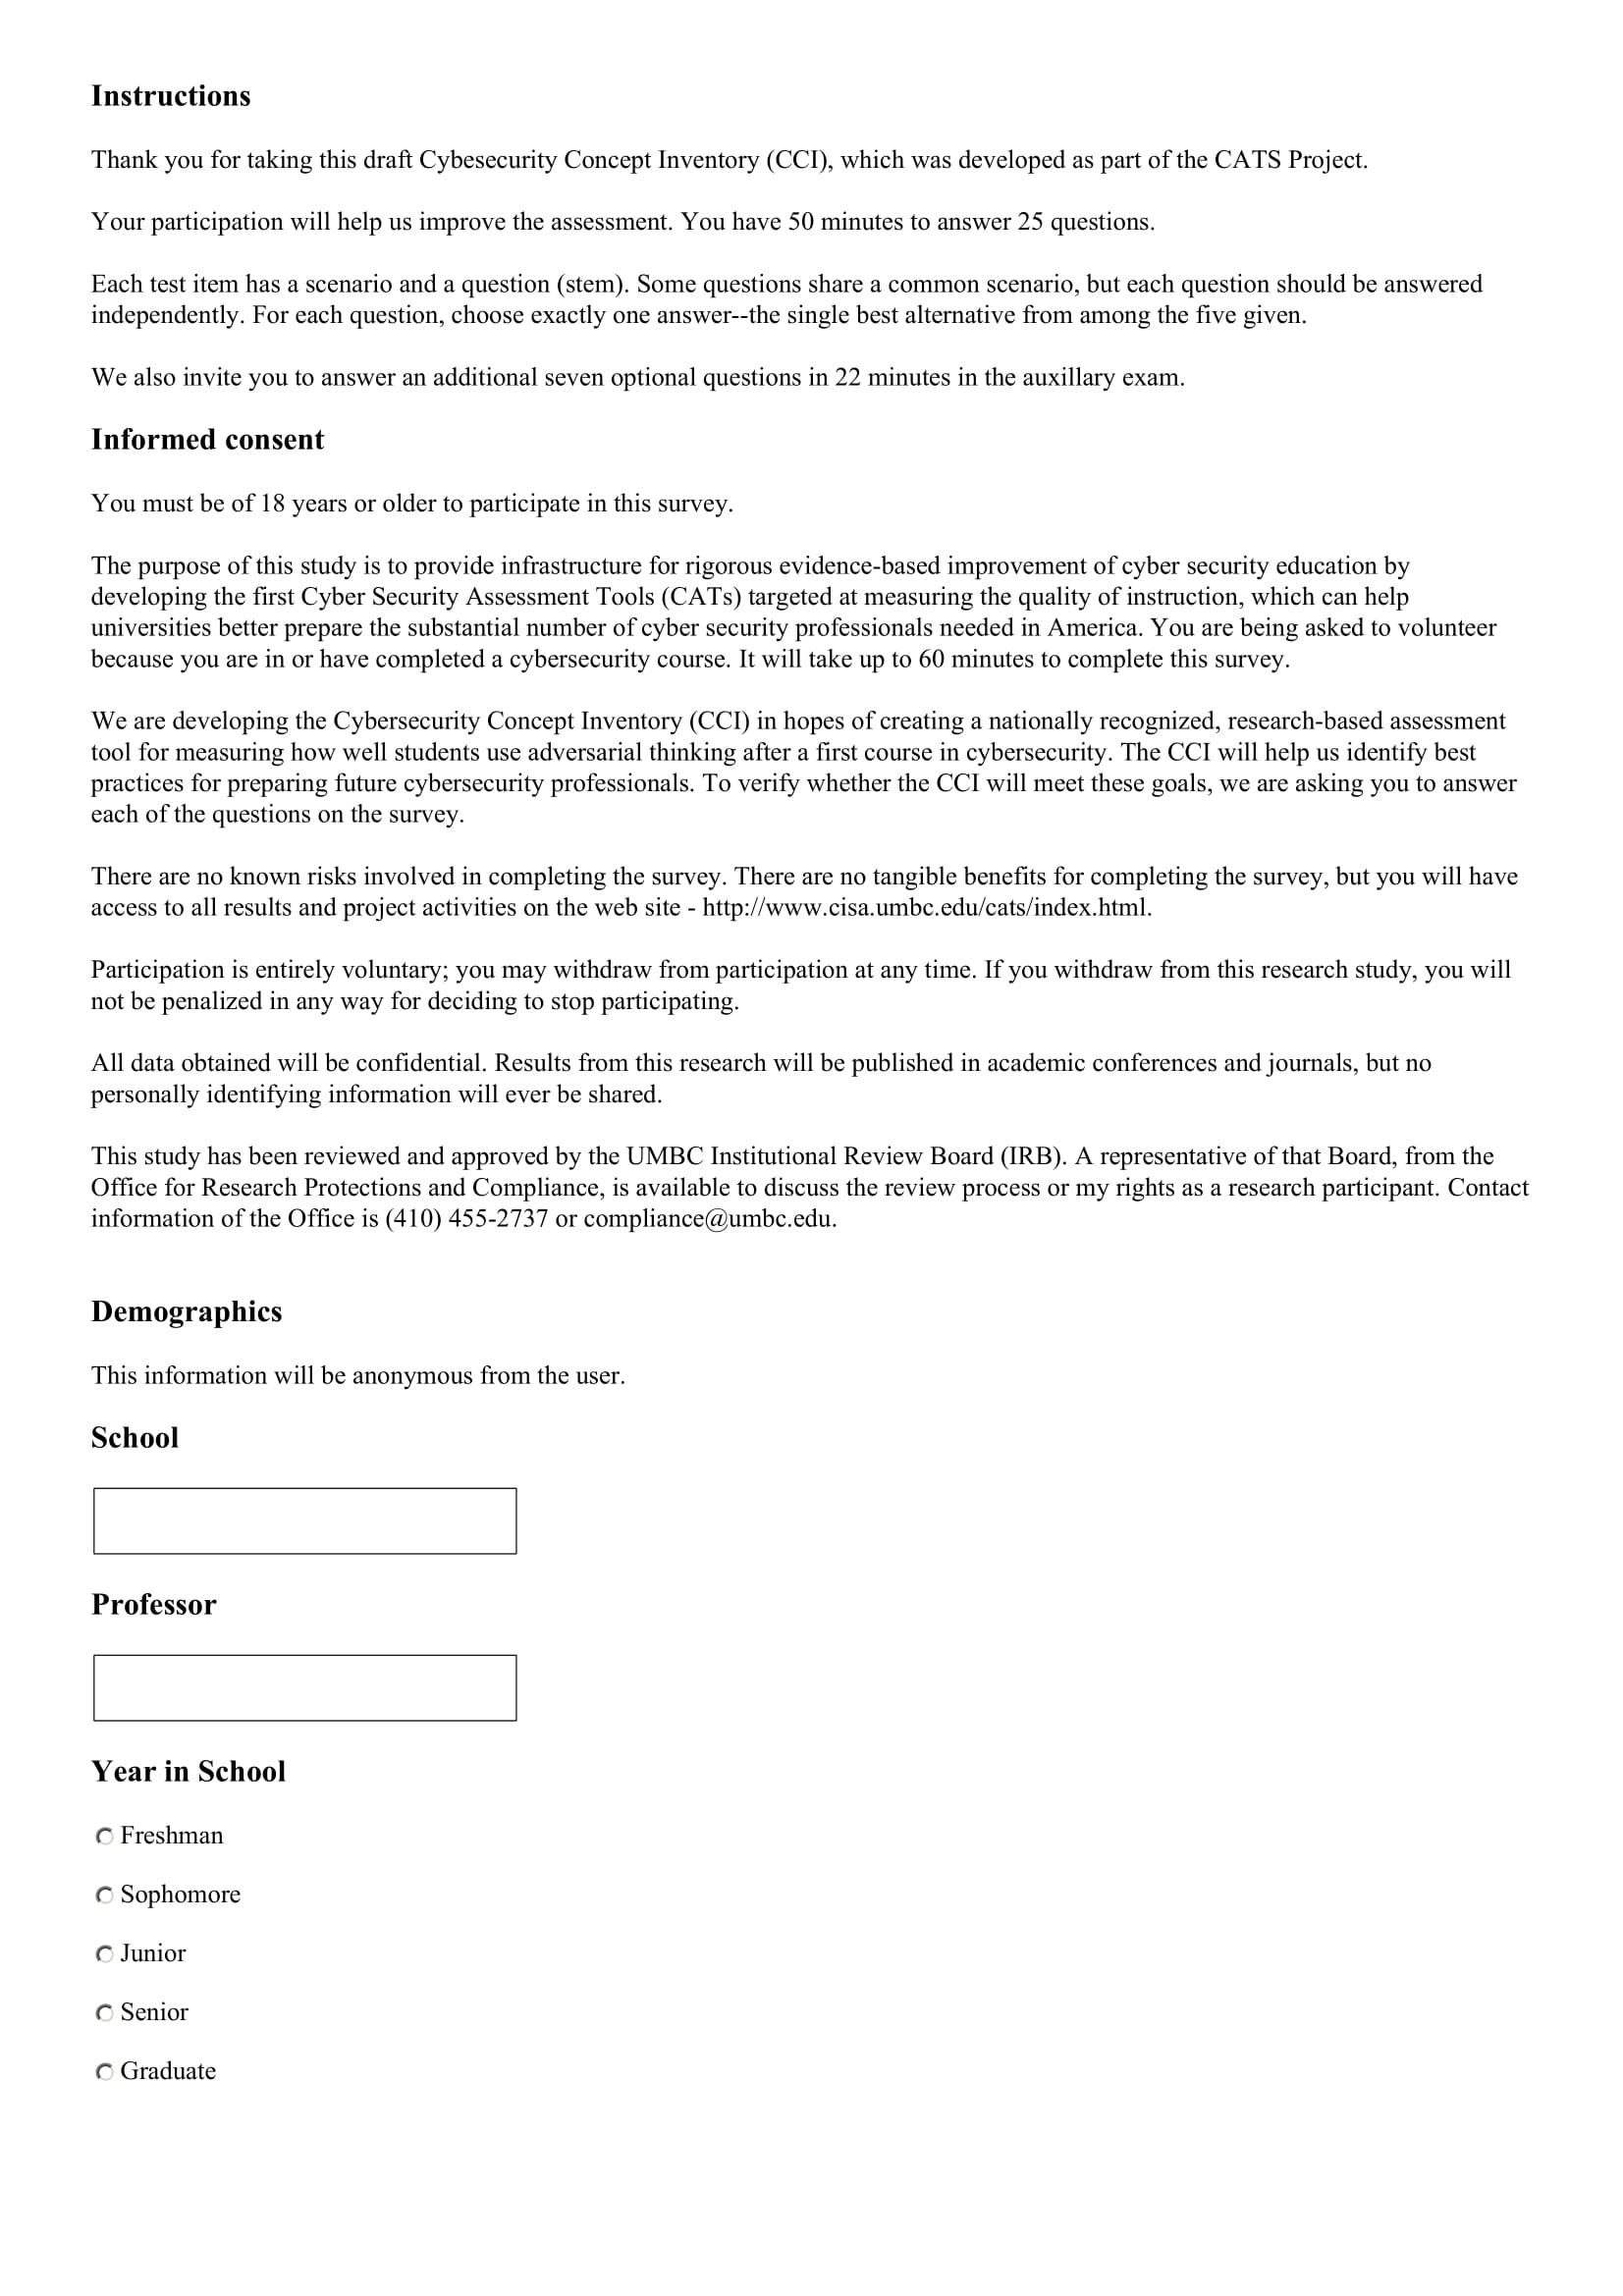
\includegraphics[scale=.25]{images/exam/correctly_formated_exam-01.jpg}
    \label{fig:correctly_formated_exam-01}
\end{center}
\end{figure}

\begin{figure}[!h]
    \begin{center}
    \advance\leftskip-3cm
    \advance\rightskip-3cm
    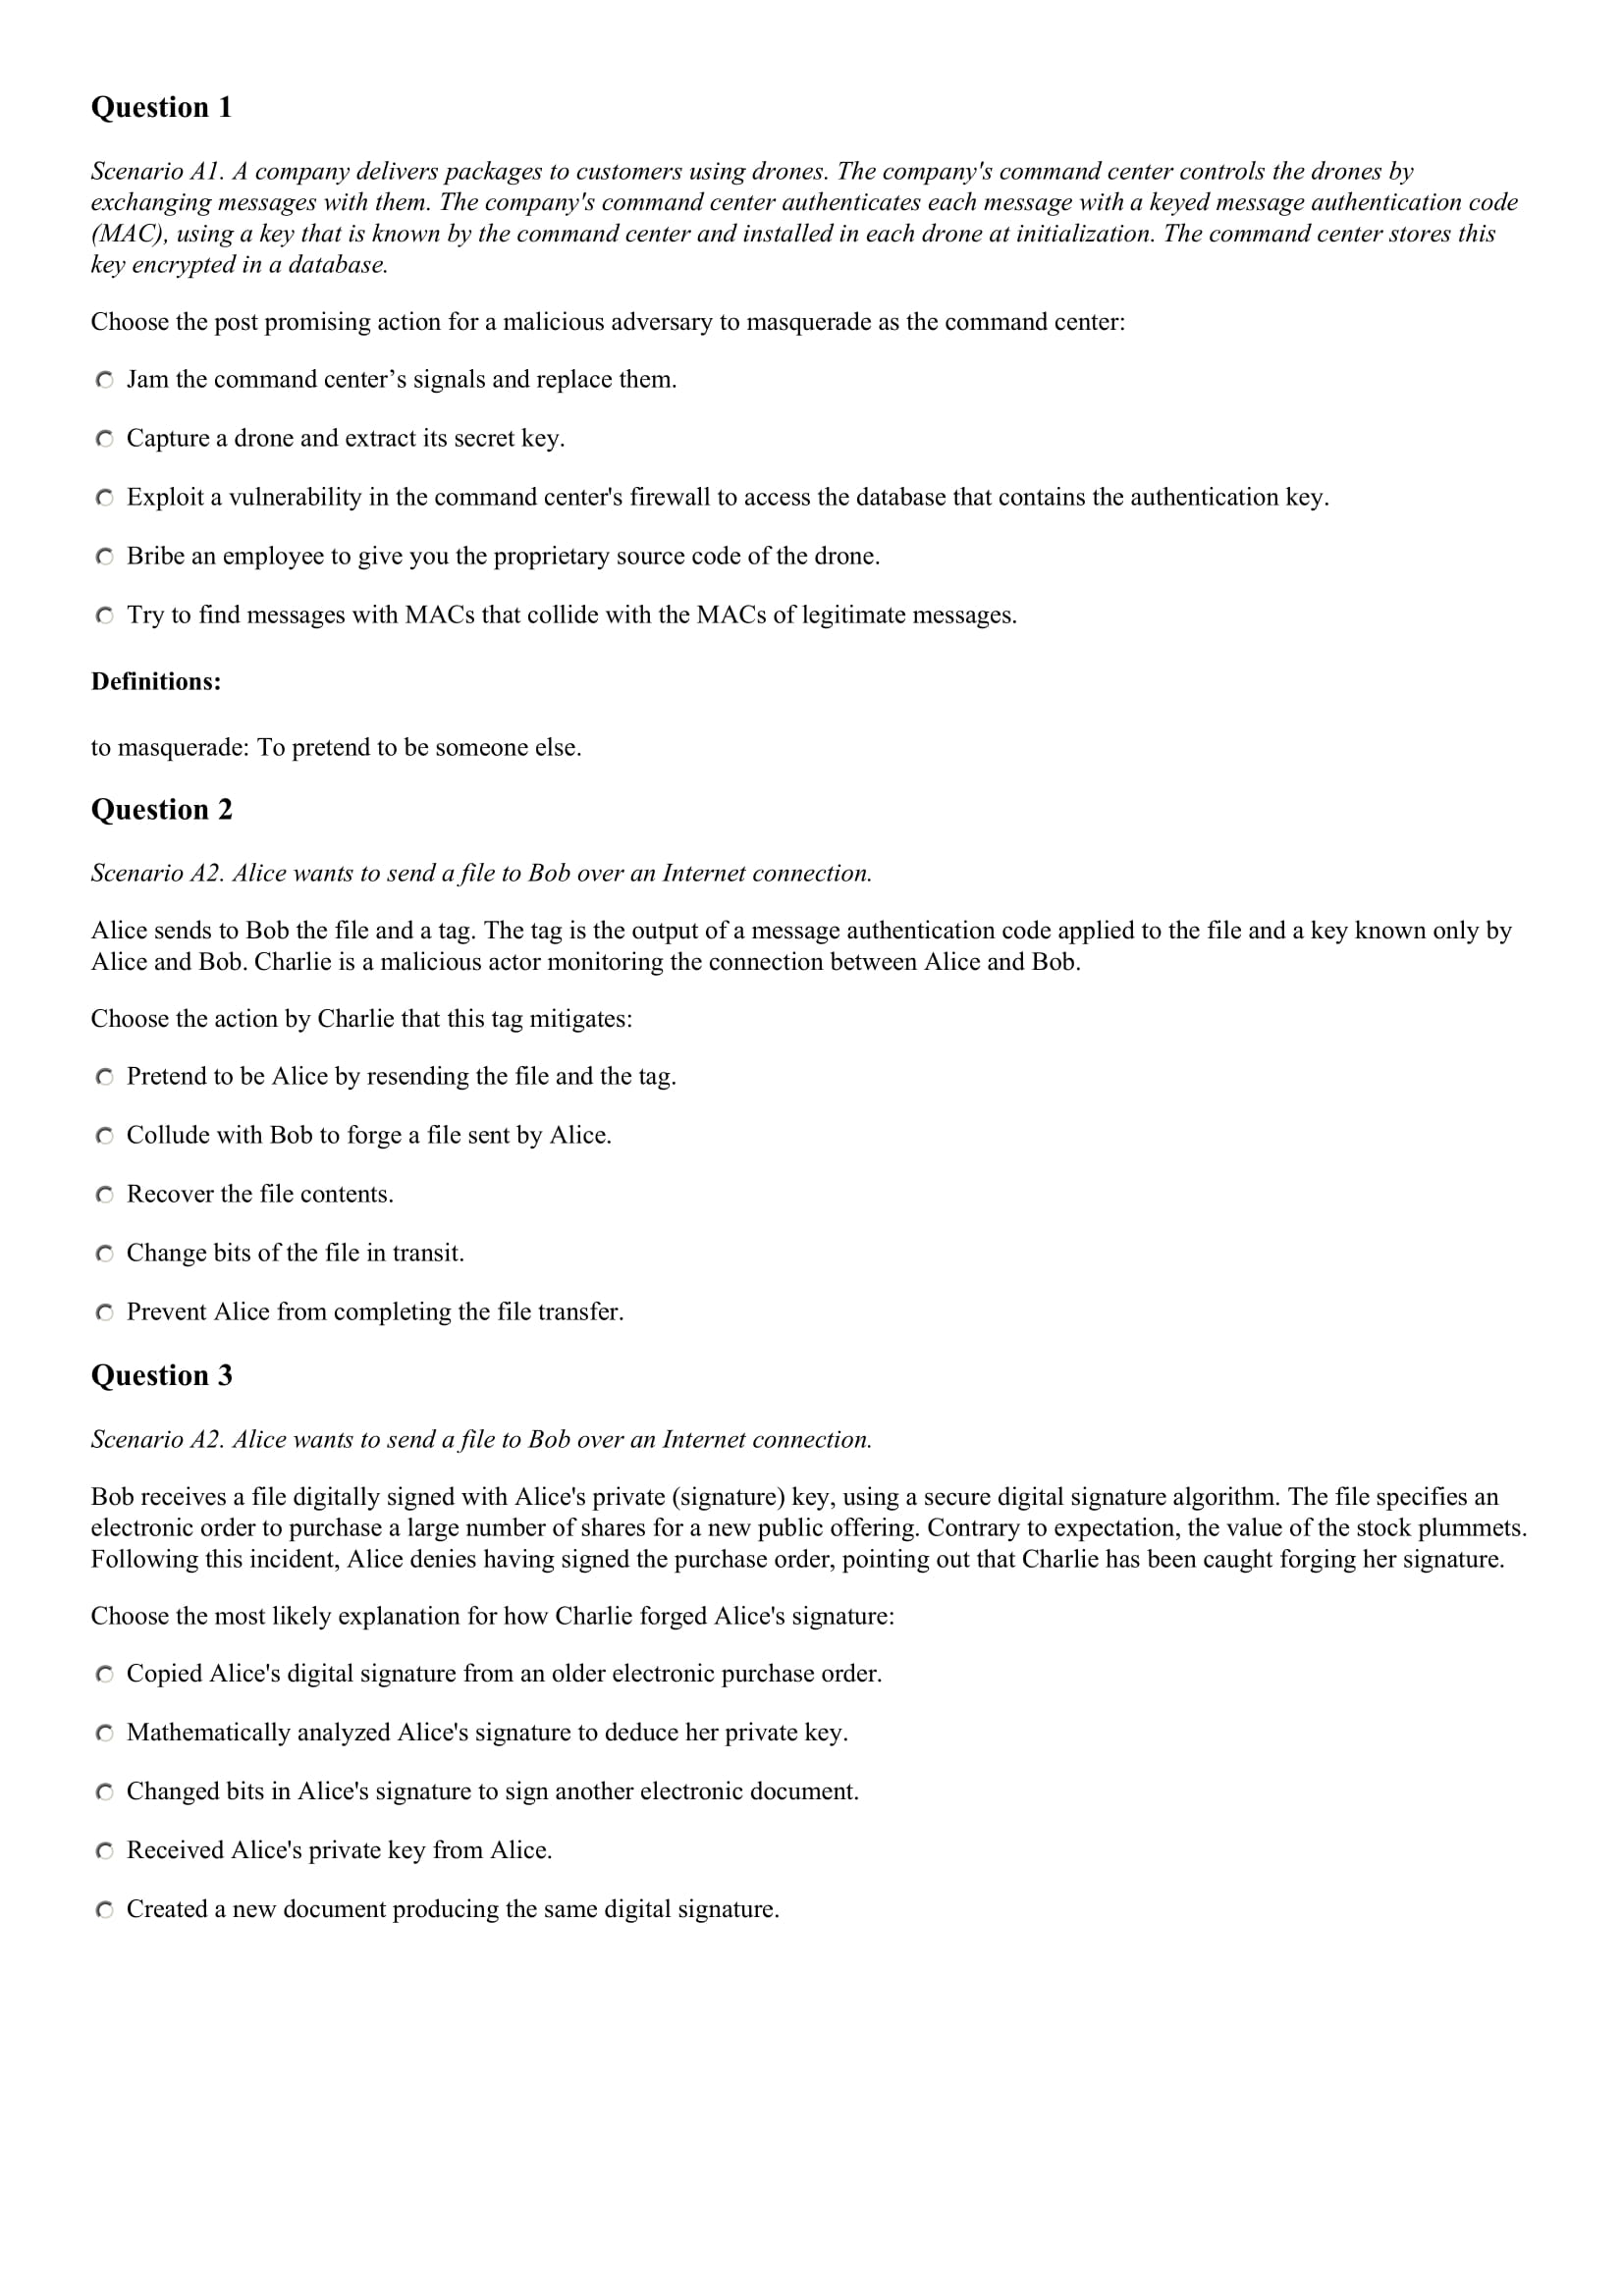
\includegraphics[scale=.25]{images/exam/correctly_formated_exam-02.jpg}
    \label{fig:correctly_formated_exam-02}
\end{center}
\end{figure}

\begin{figure}[!h]
    \begin{center}
    \advance\leftskip-3cm
    \advance\rightskip-3cm
    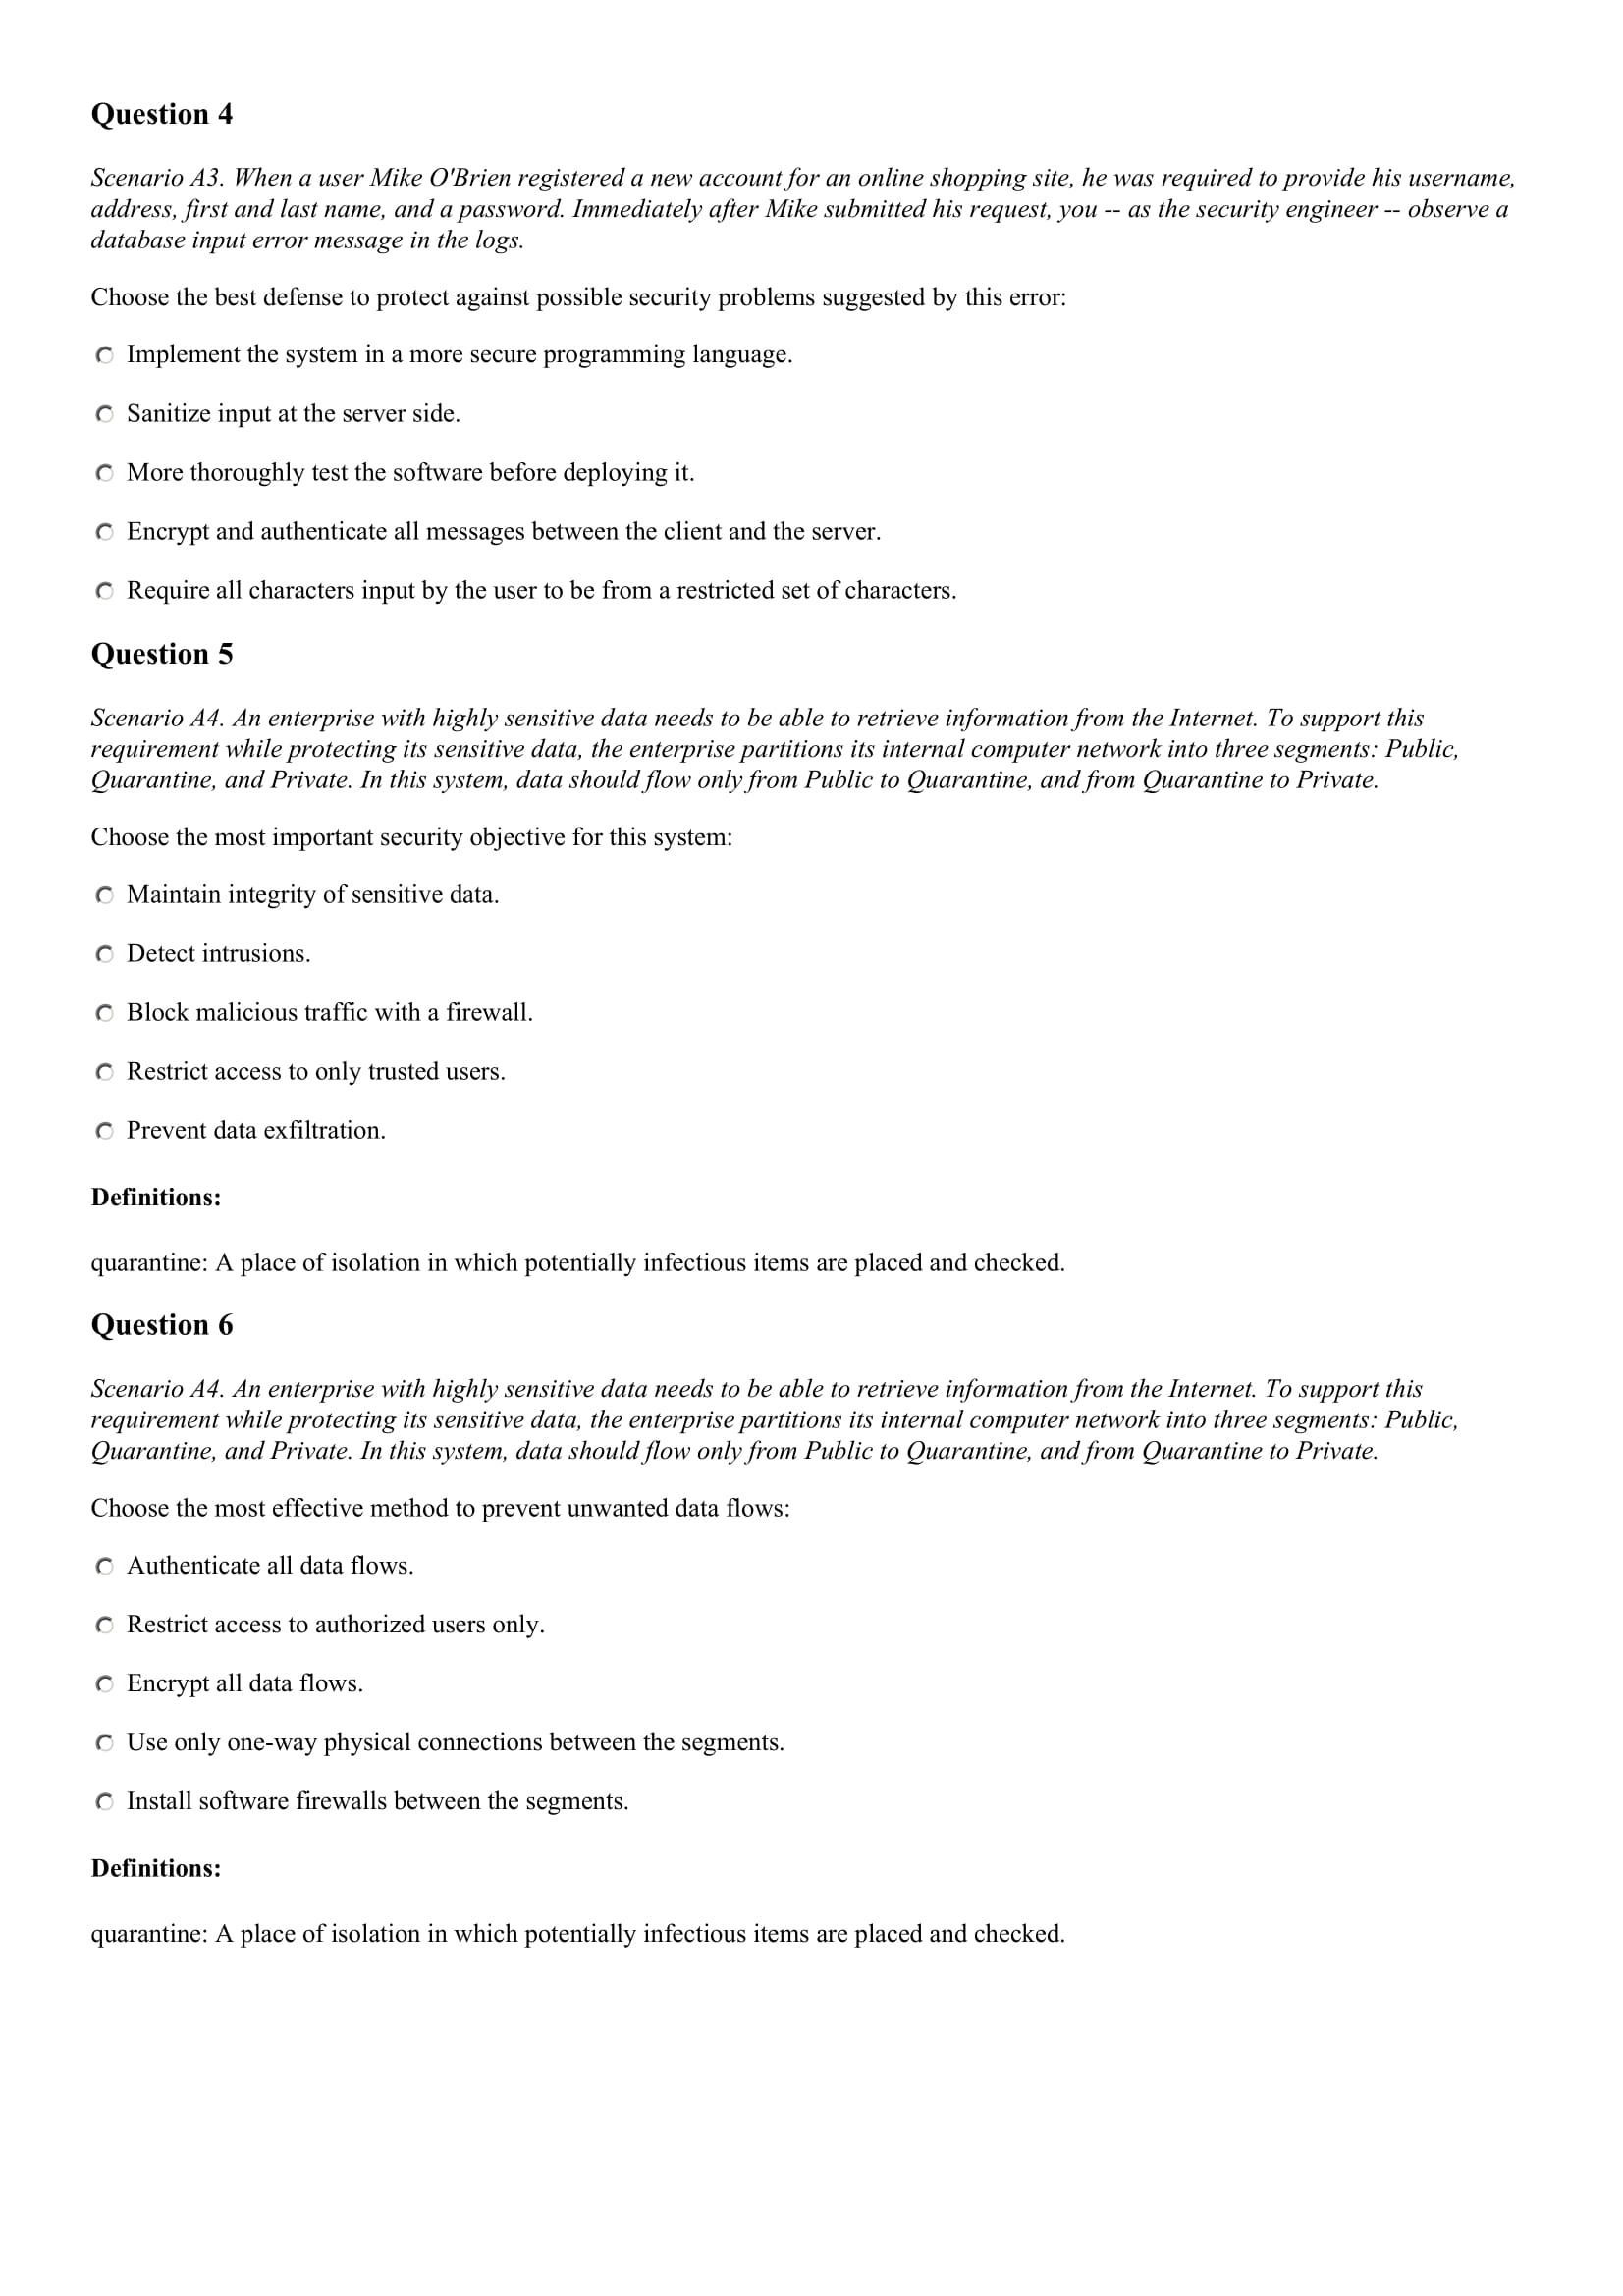
\includegraphics[scale=.25]{images/exam/correctly_formated_exam-03.jpg}
    \label{fig:correctly_formated_exam-03}
\end{center}
\end{figure}
\begin{figure}[!h]
    \begin{center}
    \advance\leftskip-3cm
    \advance\rightskip-3cm
    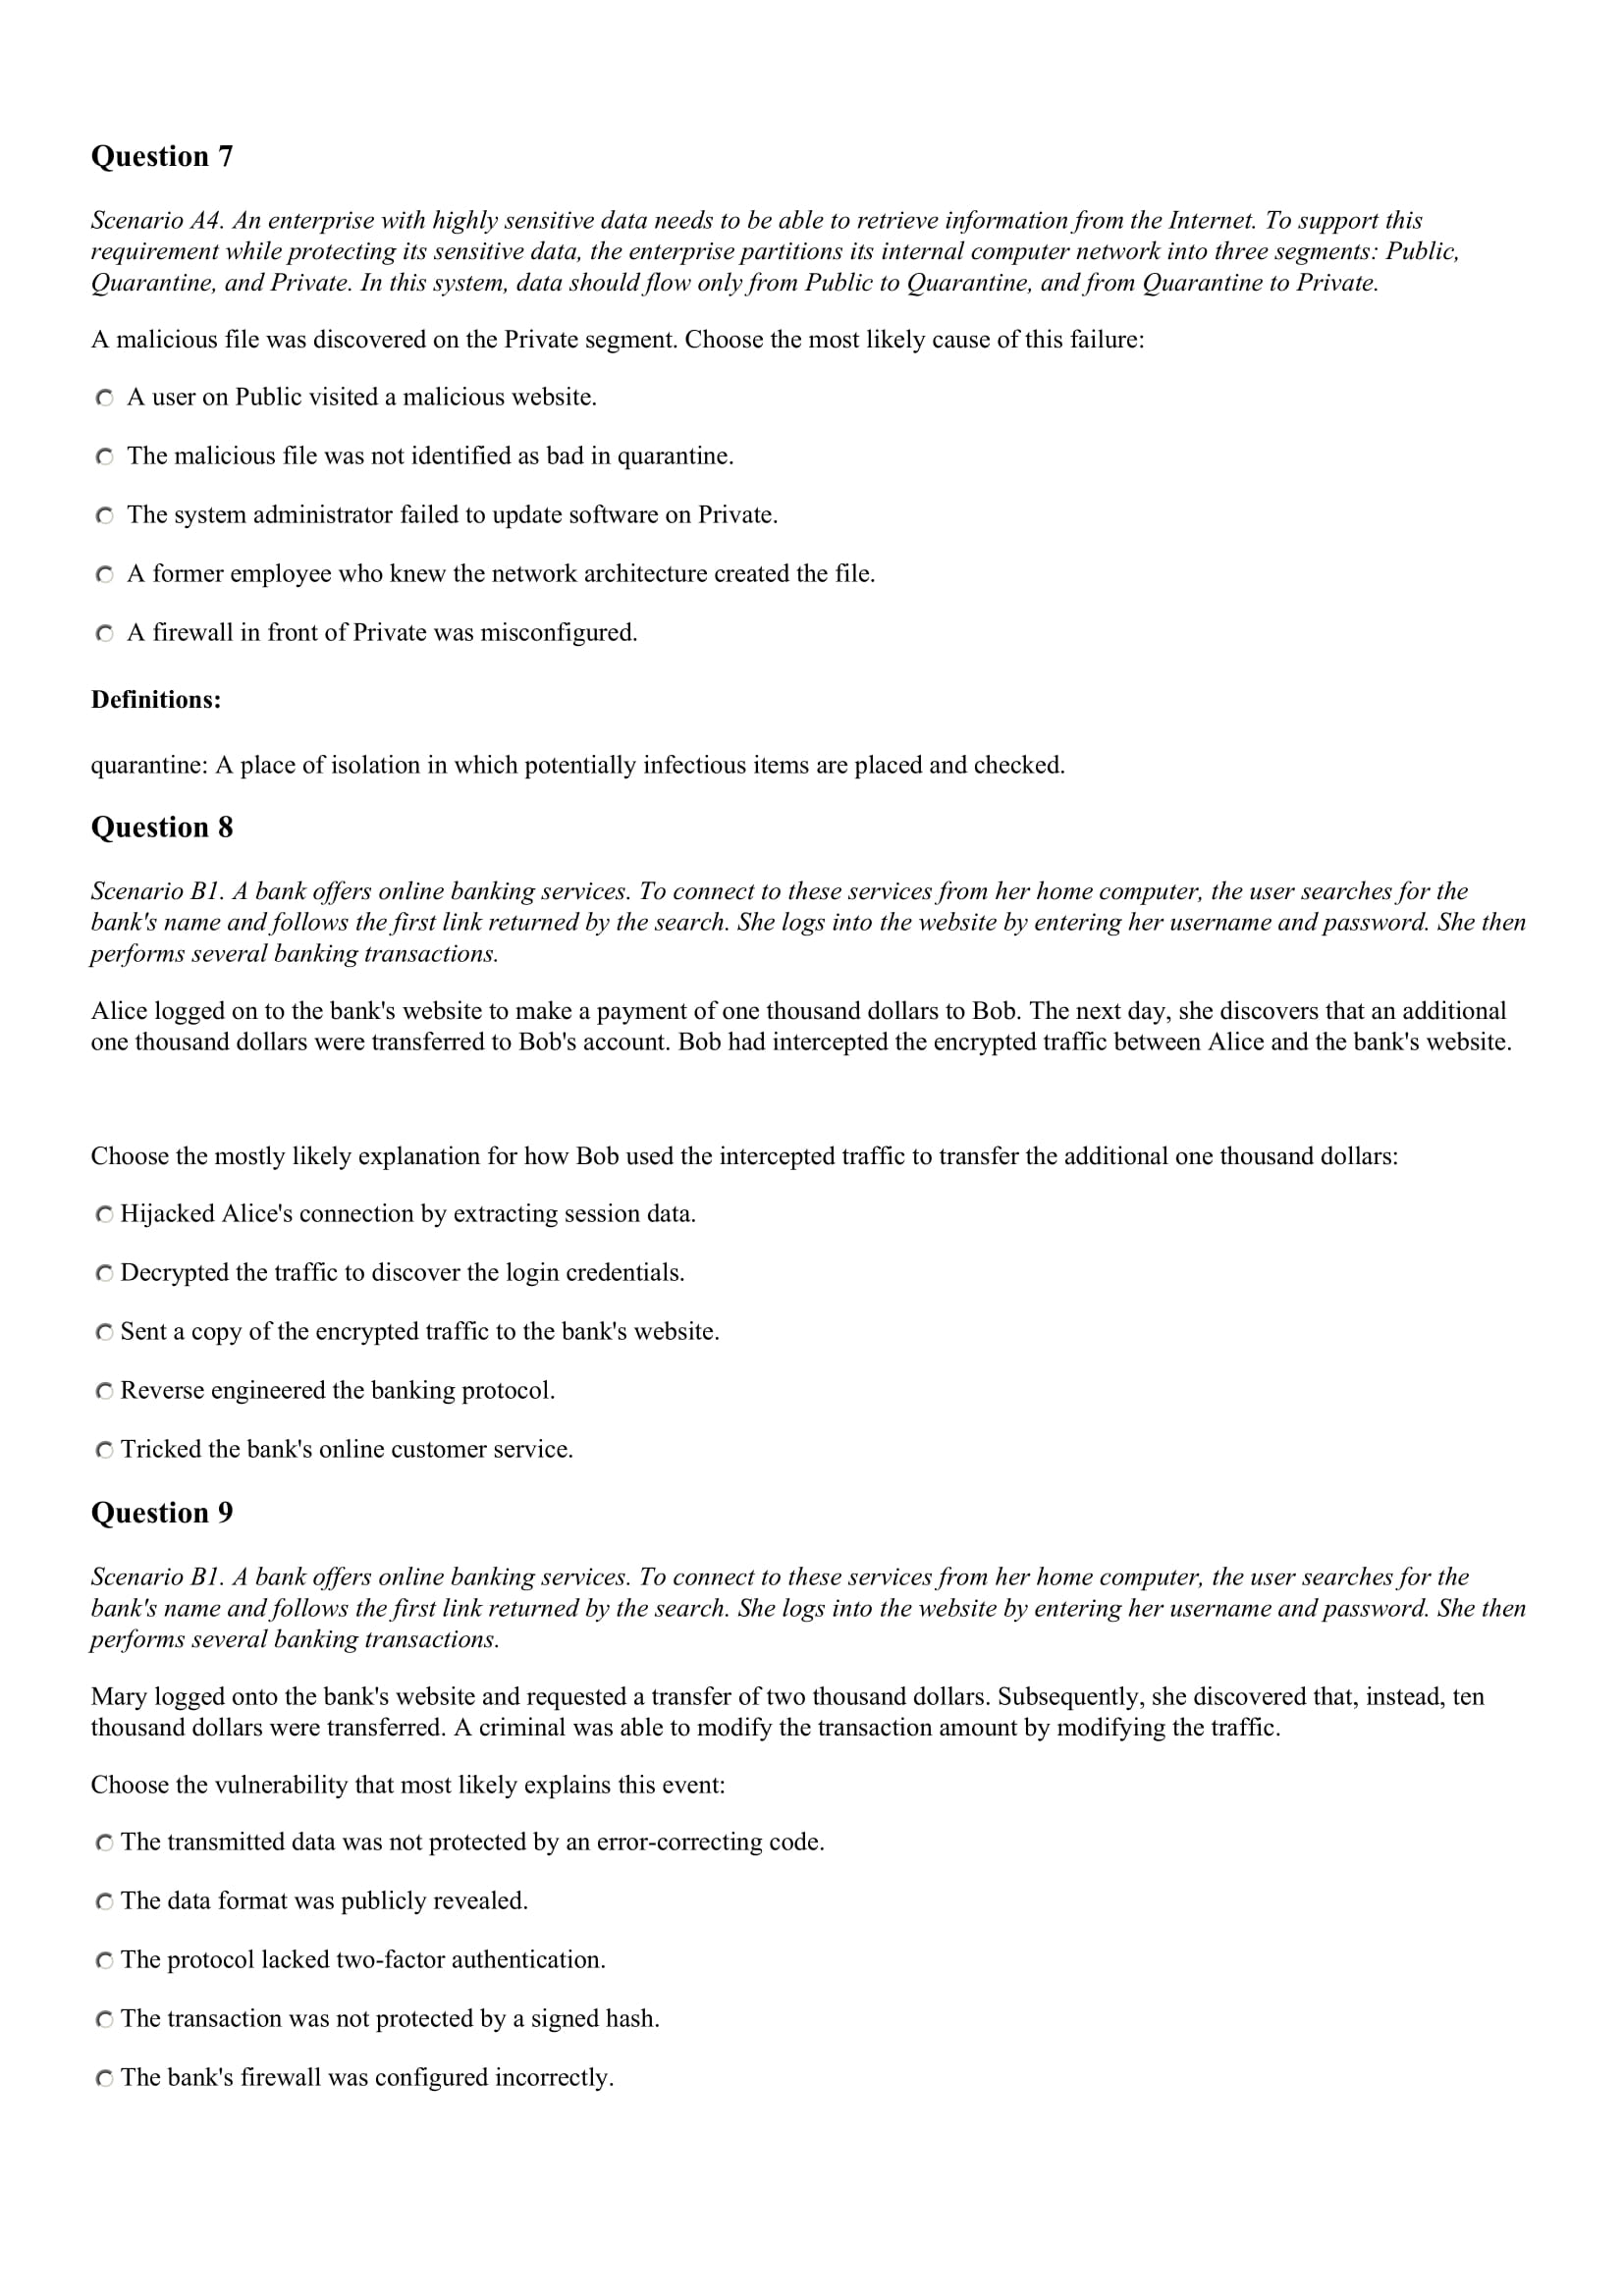
\includegraphics[scale=.25]{images/exam/correctly_formated_exam-04.jpg}
    \label{fig:correctly_formated_exam-04}
\end{center}
\end{figure}
\begin{figure}[!h]
    \begin{center}
    \advance\leftskip-3cm
    \advance\rightskip-3cm
    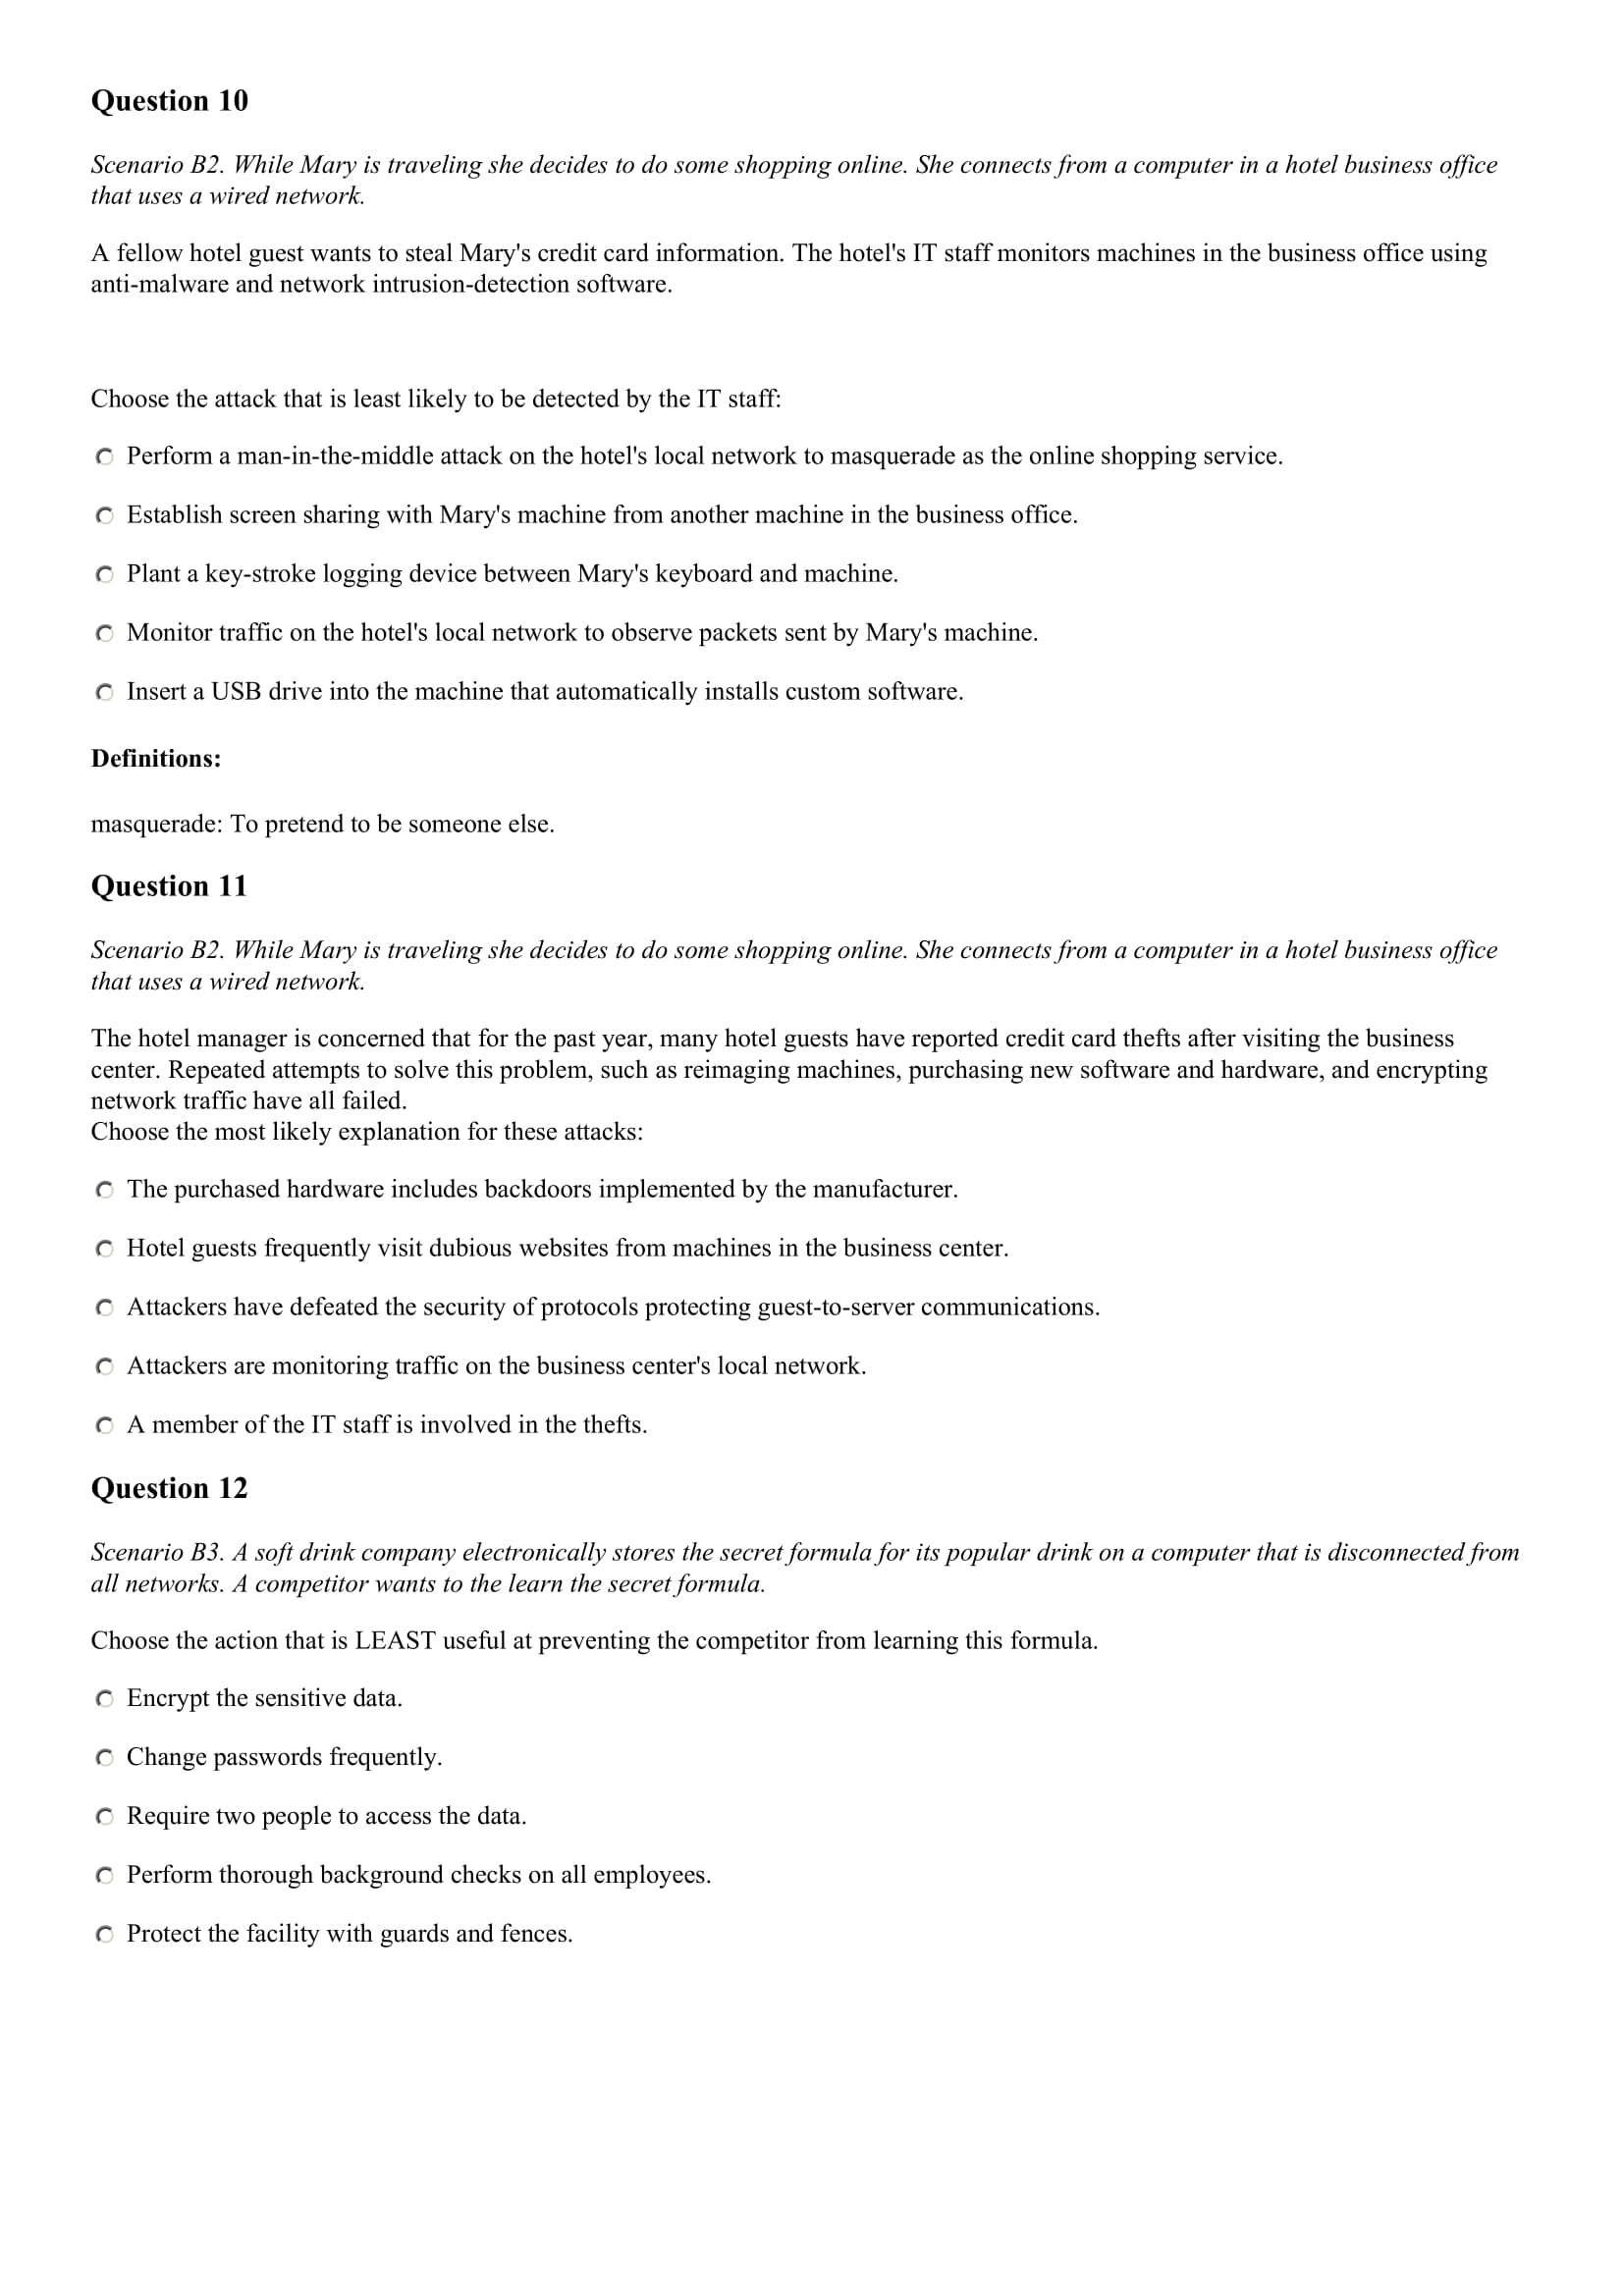
\includegraphics[scale=.25]{images/exam/correctly_formated_exam-05.jpg}
    \label{fig:correctly_formated_exam-05}
\end{center}
\end{figure}
\begin{figure}[!h]
    \begin{center}
    \advance\leftskip-3cm
    \advance\rightskip-3cm
    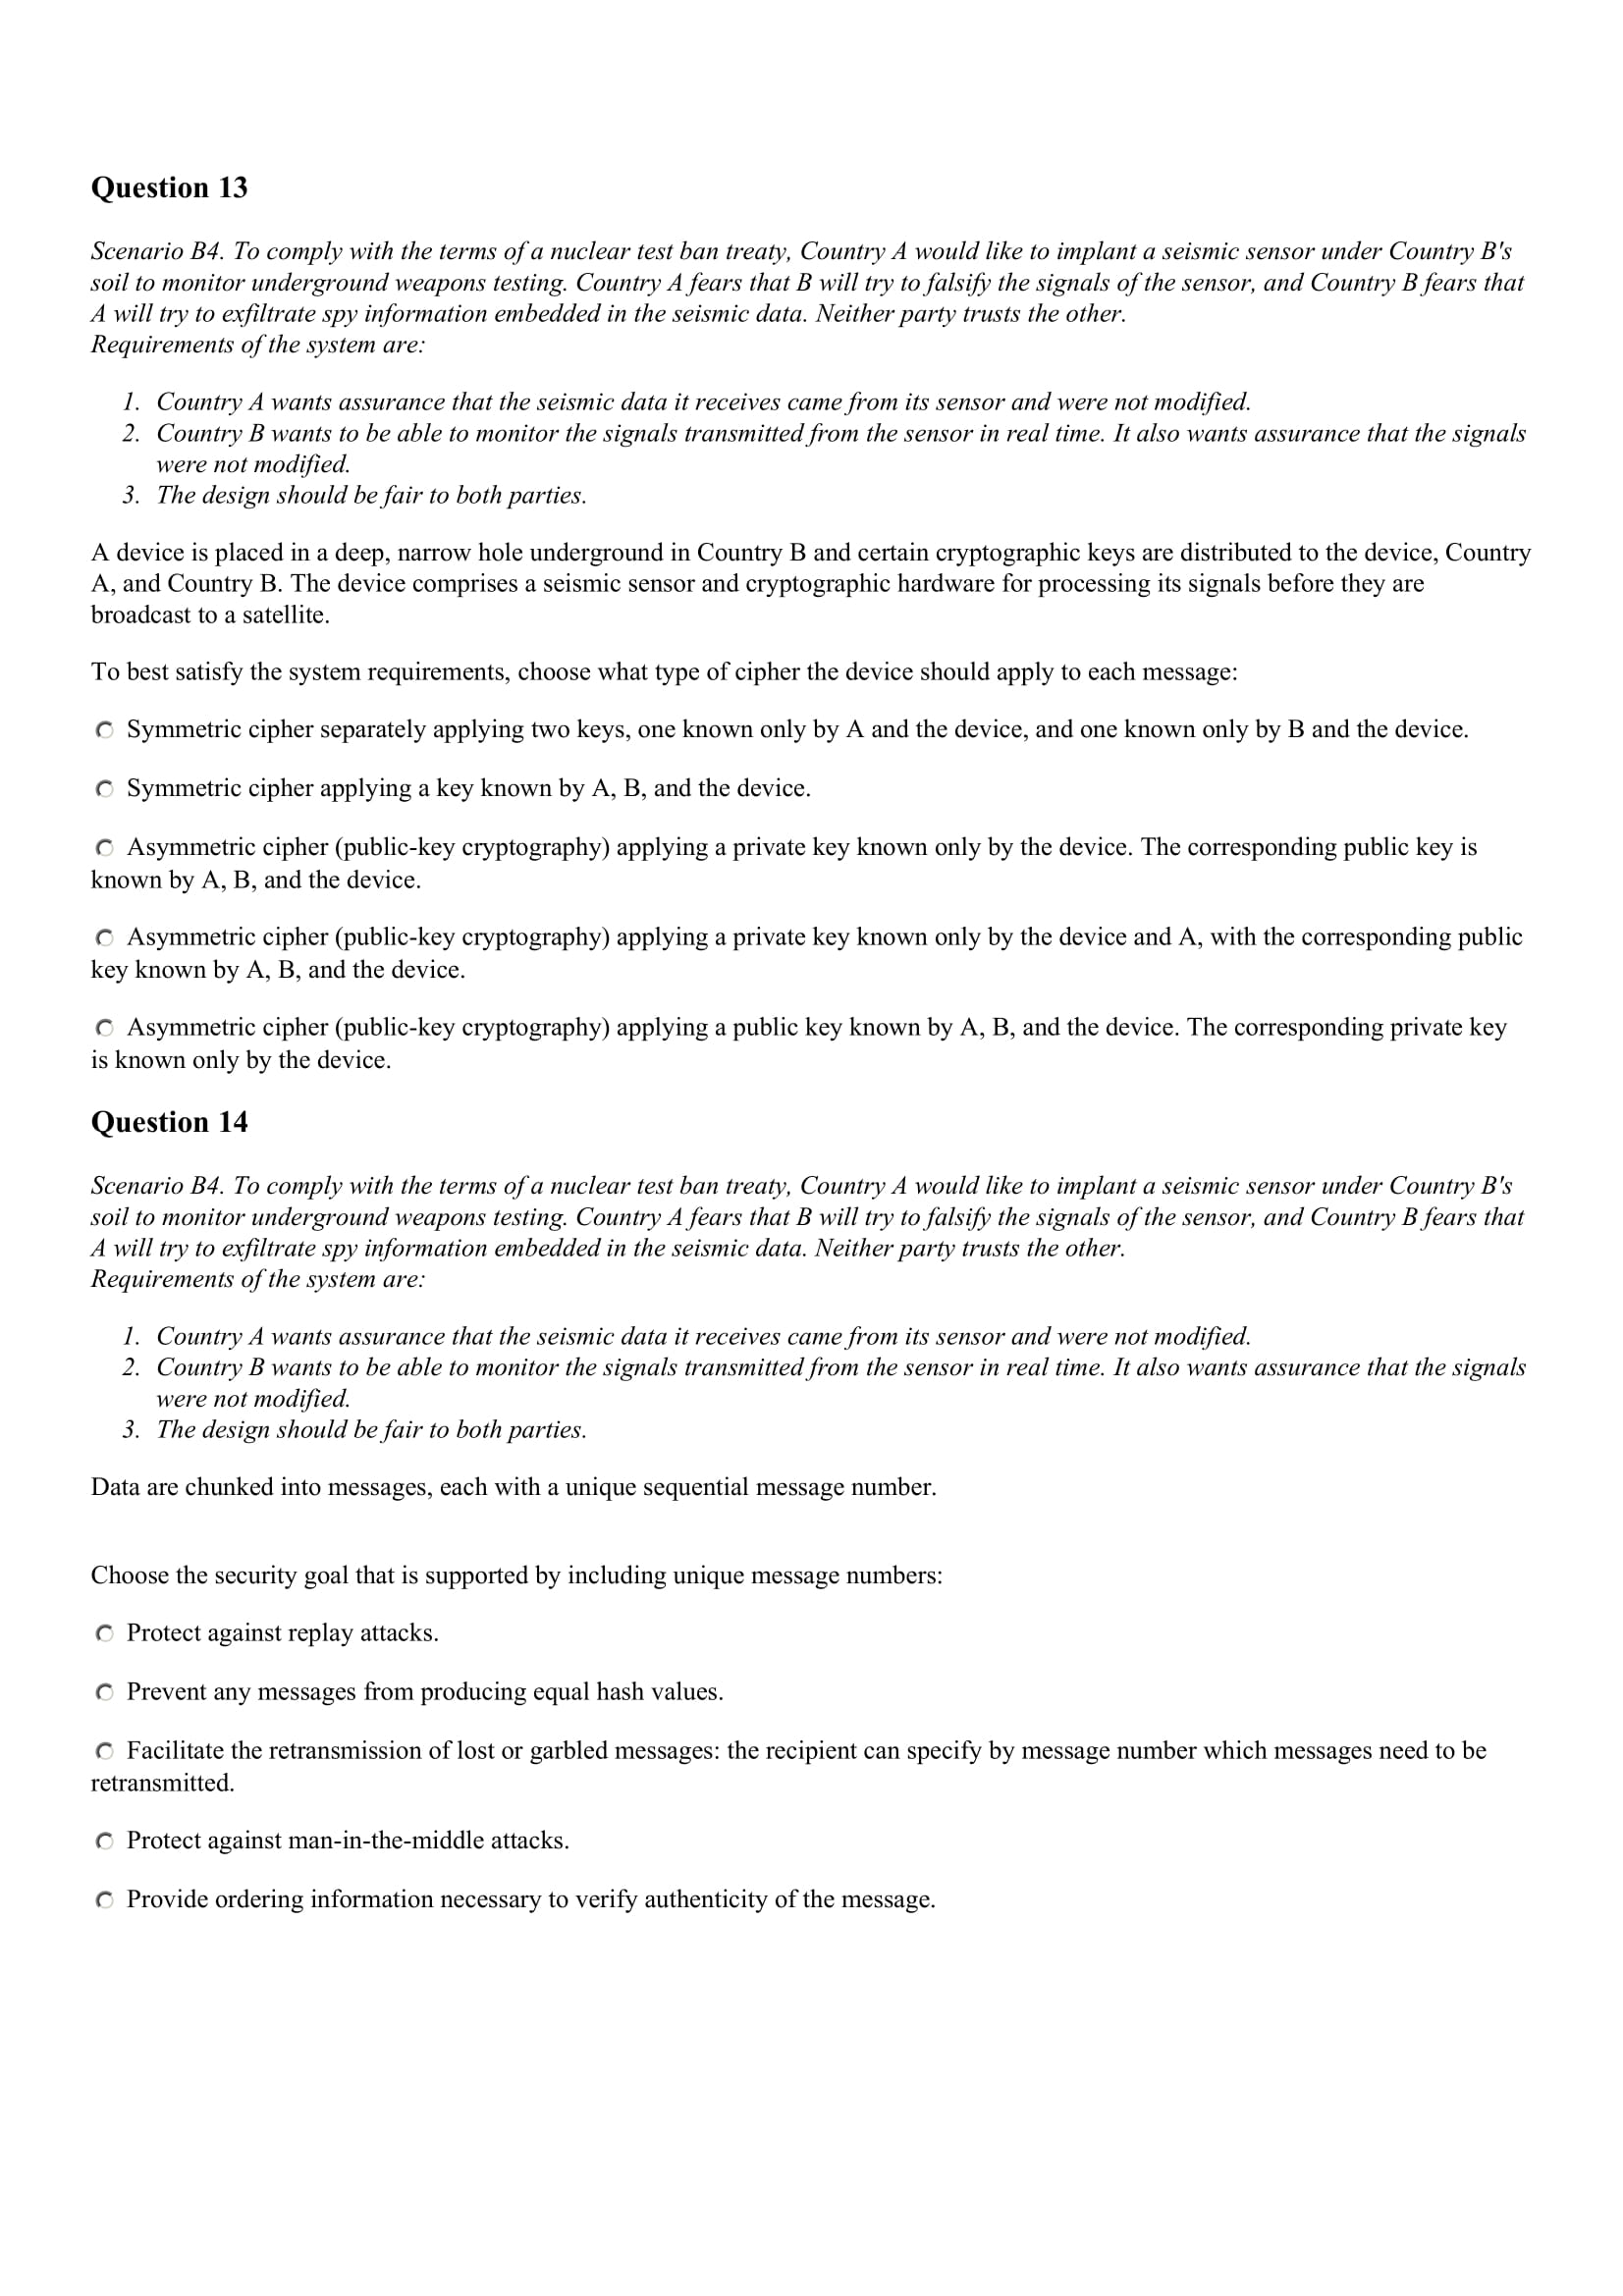
\includegraphics[scale=.25]{images/exam/correctly_formated_exam-06.jpg}
    \label{fig:correctly_formated_exam-06}
\end{center}
\end{figure}

\begin{figure}[!h]
    \begin{center}
    \advance\leftskip-3cm
    \advance\rightskip-3cm
    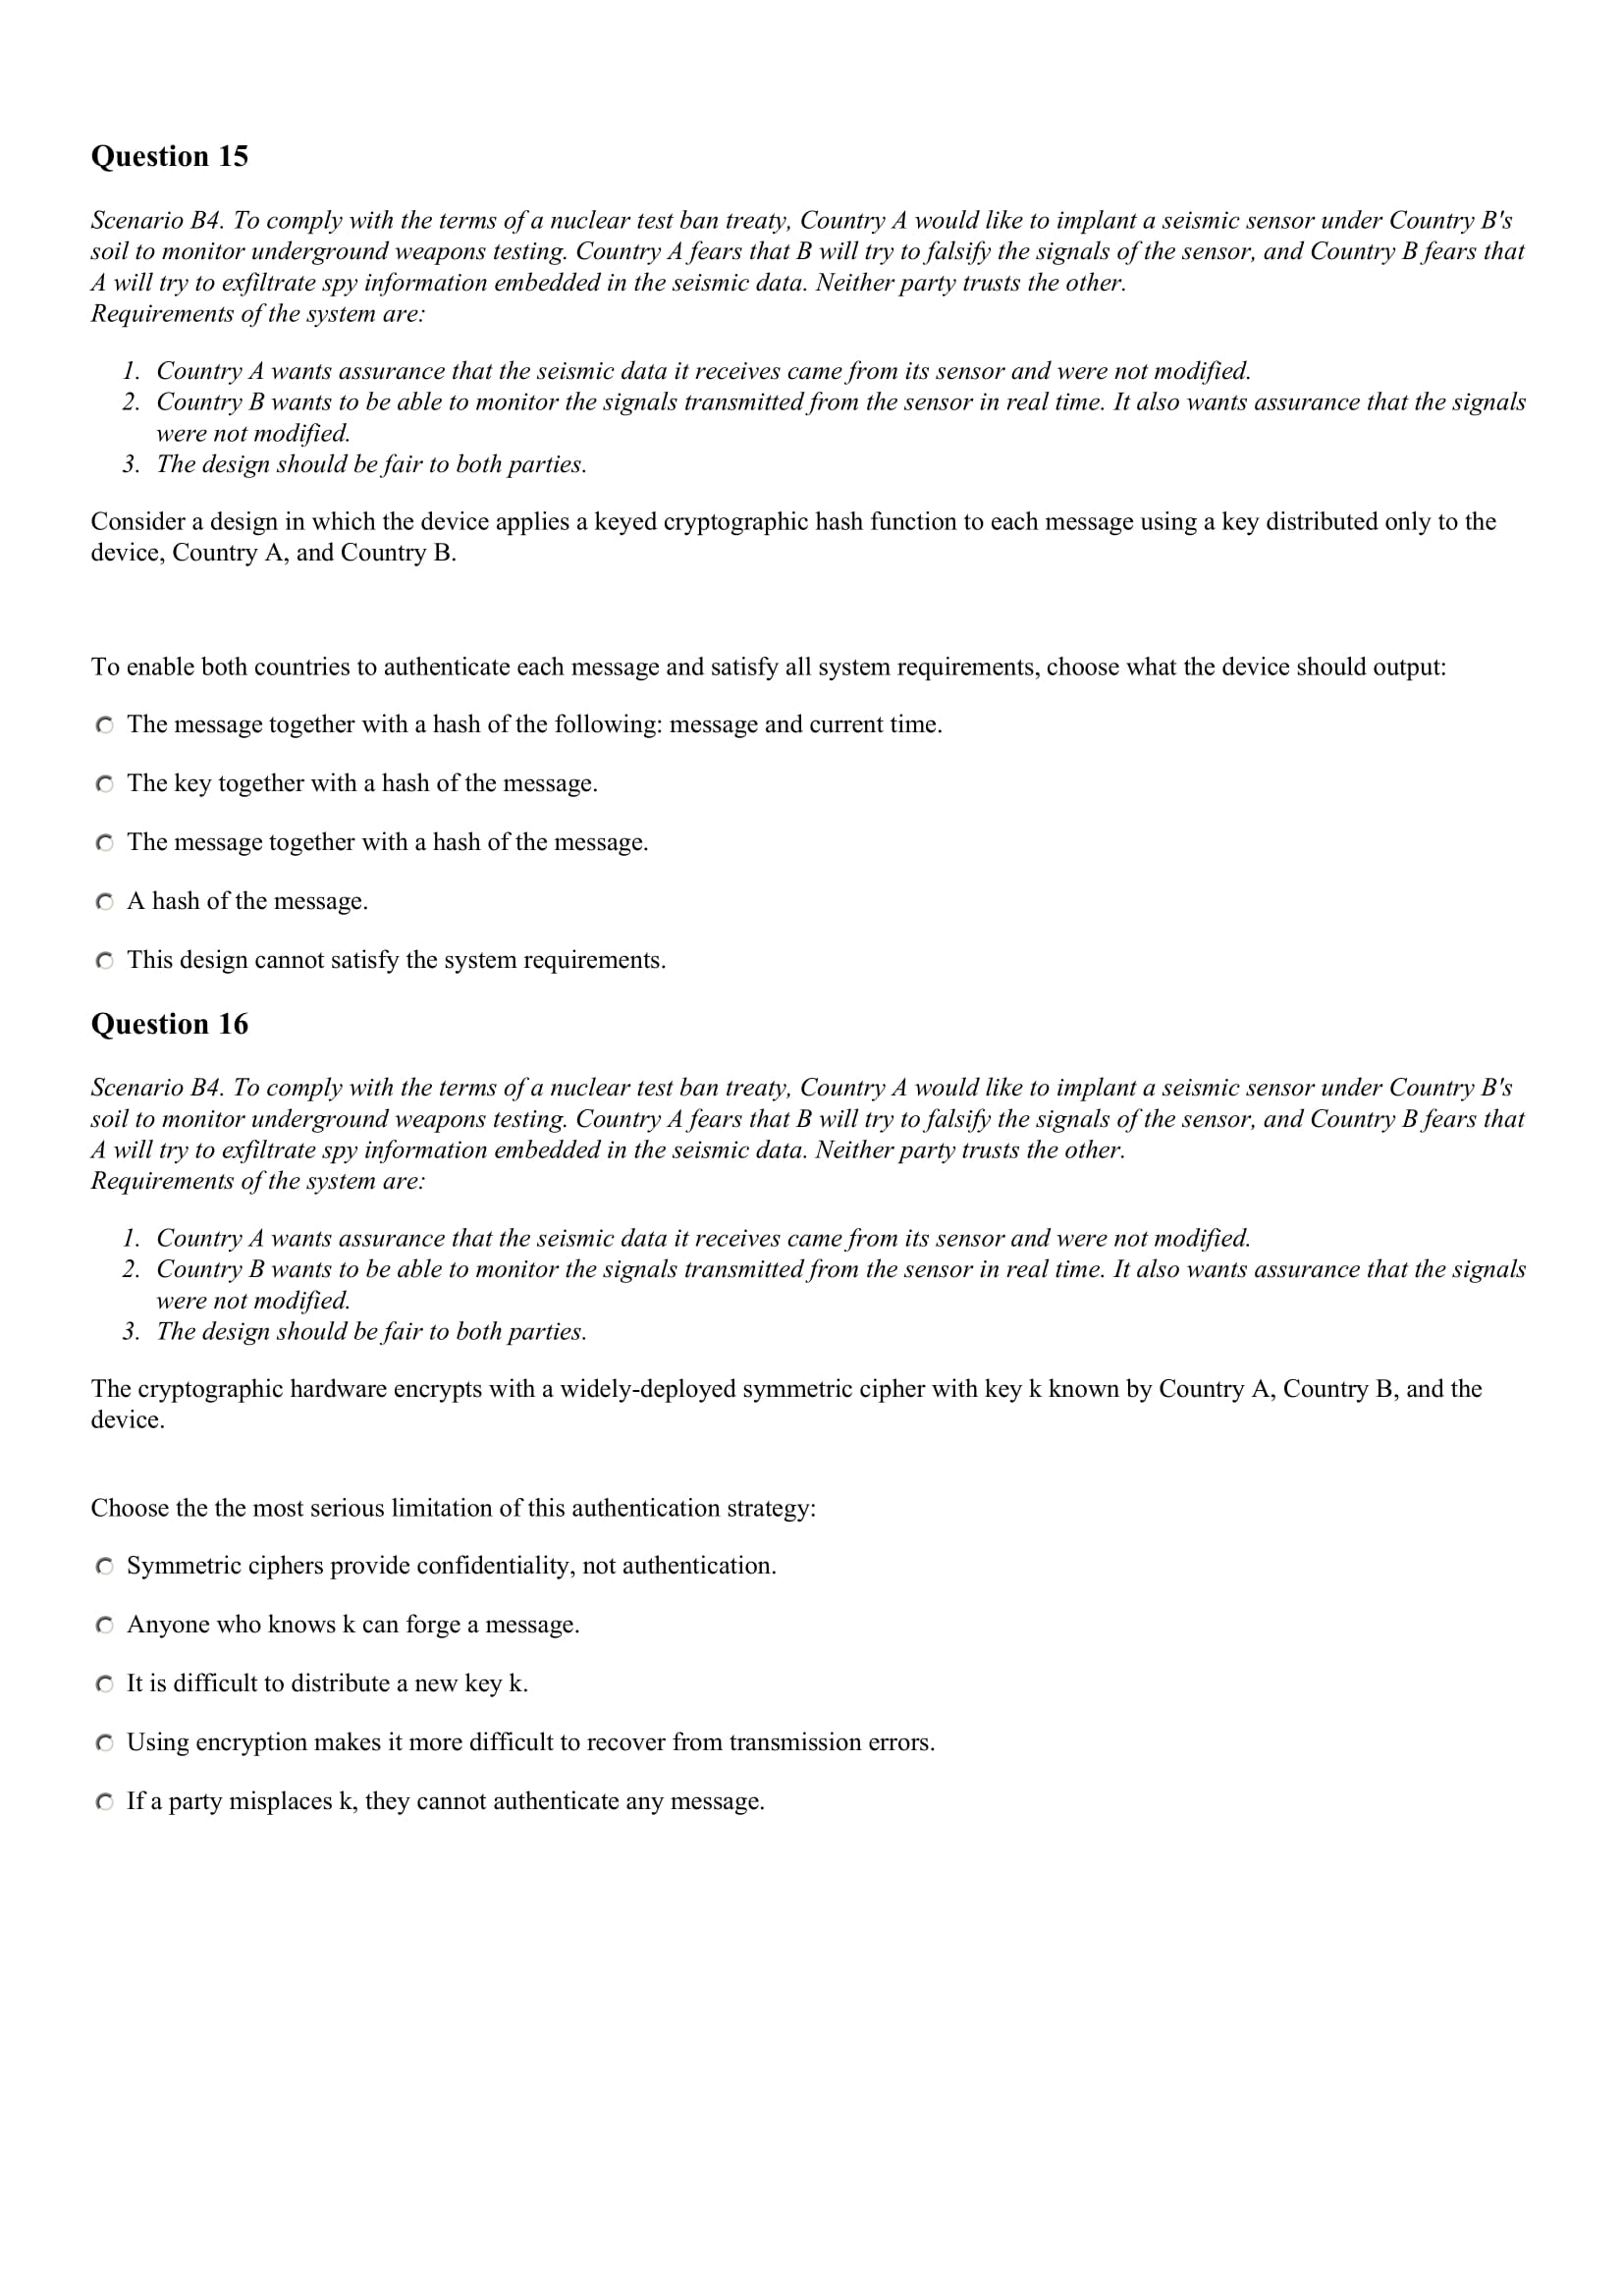
\includegraphics[scale=.25]{images/exam/correctly_formated_exam-07.jpg}
    \label{fig:correctly_formated_exam-07}
\end{center}
\end{figure}

\begin{figure}[!h]
    \begin{center}
    \advance\leftskip-3cm
    \advance\rightskip-3cm
    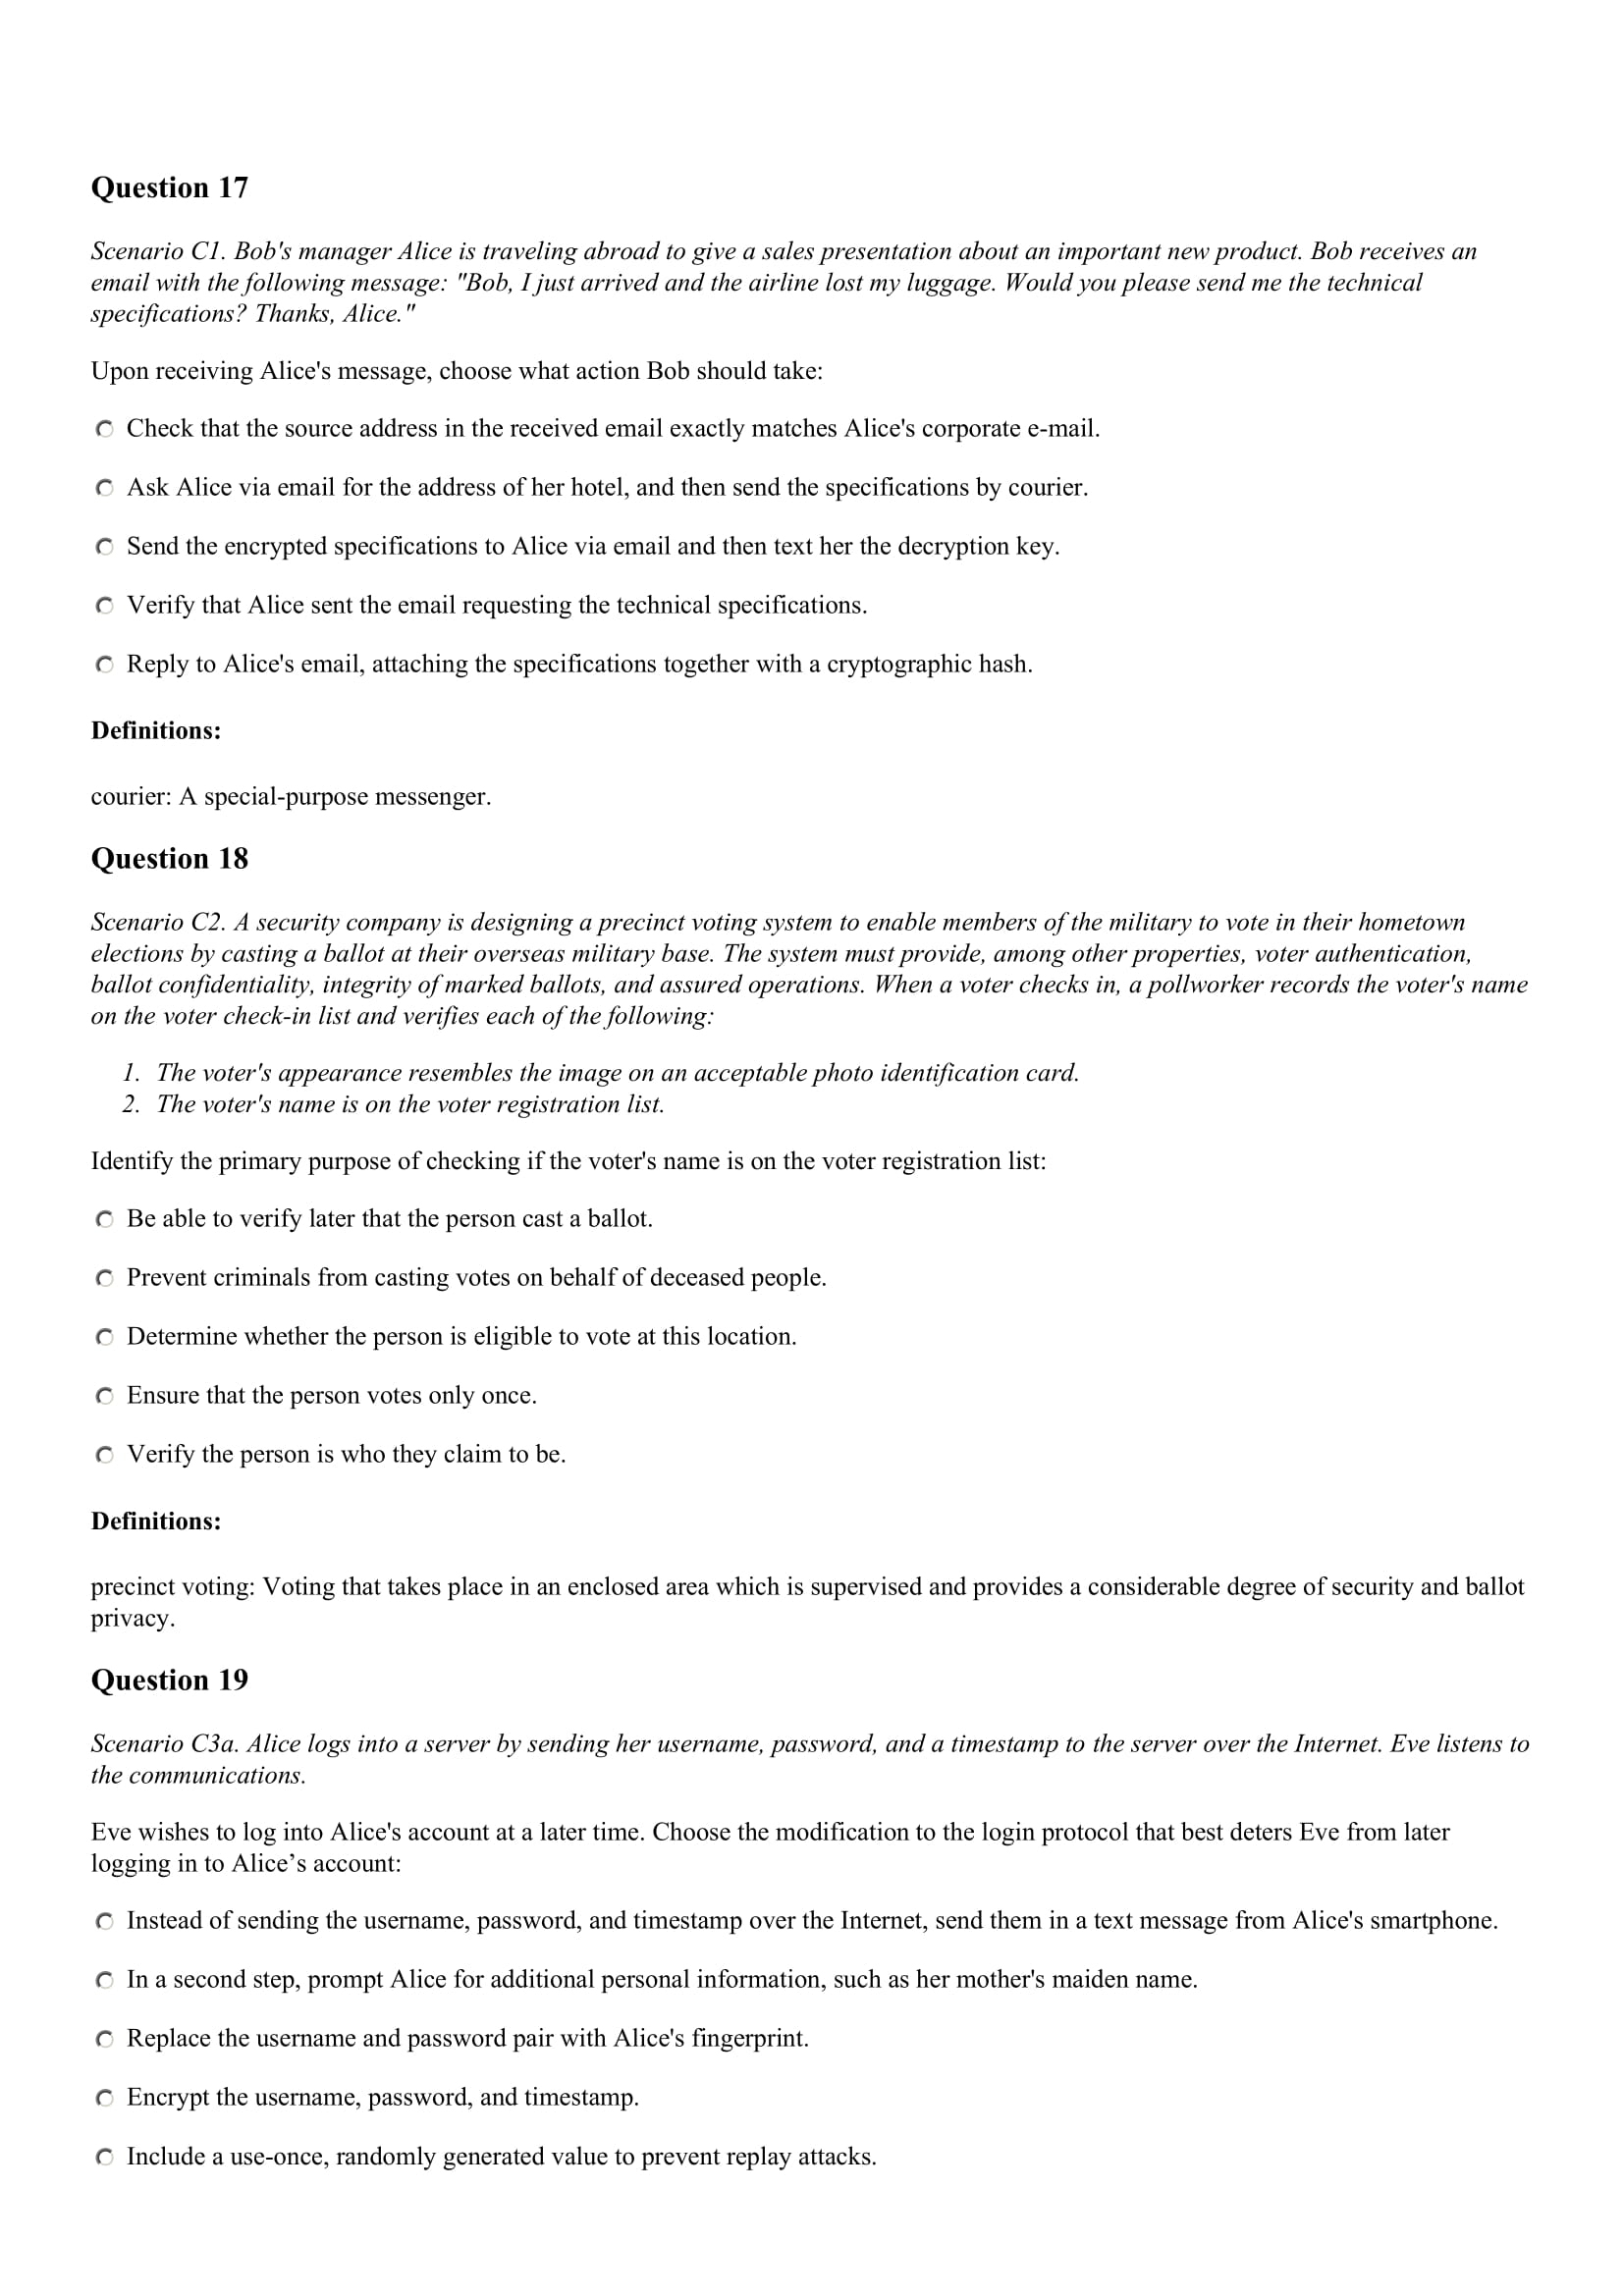
\includegraphics[scale=.25]{images/exam/correctly_formated_exam-08.jpg}
    \label{fig:correctly_formated_exam-08}
\end{center}
\end{figure}

\begin{figure}[!h]
    \begin{center}
    \advance\leftskip-3cm
    \advance\rightskip-3cm
    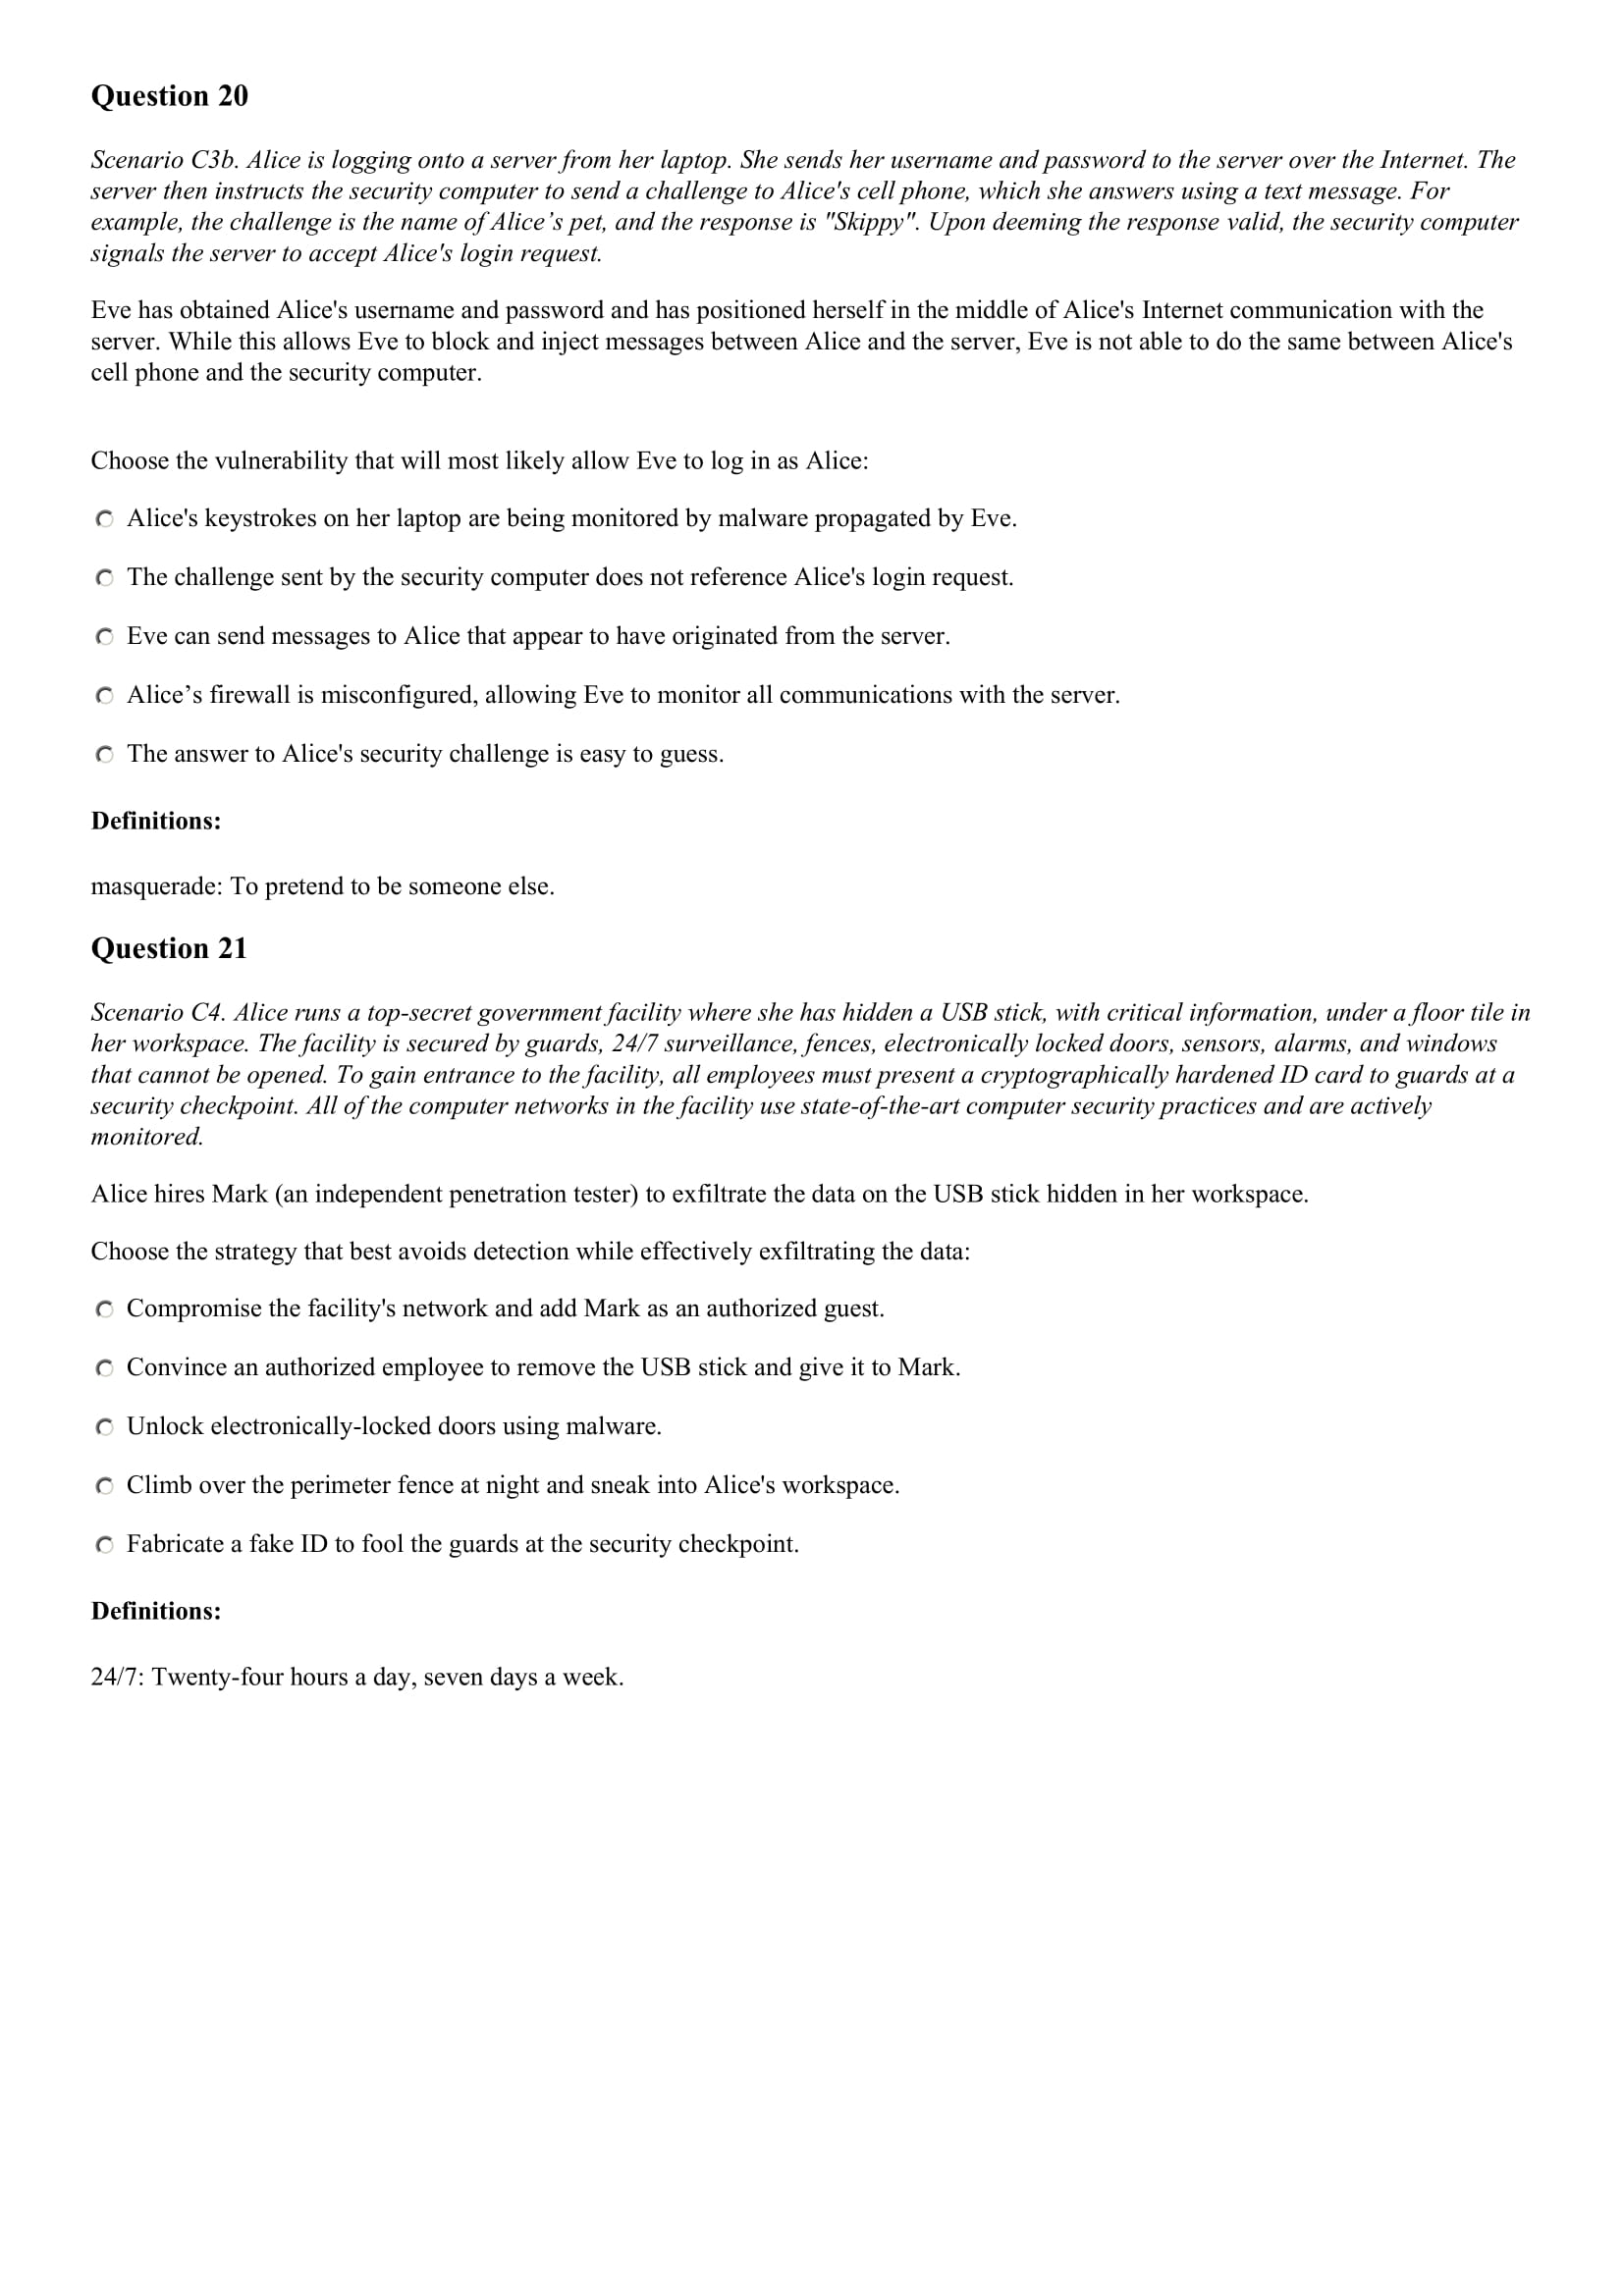
\includegraphics[scale=.25]{images/exam/correctly_formated_exam-09.jpg}
    \label{fig:correctly_formated_exam-09}
\end{center}
\end{figure}

\begin{figure}[!h]
    \begin{center}
    \advance\leftskip-3cm
    \advance\rightskip-3cm
    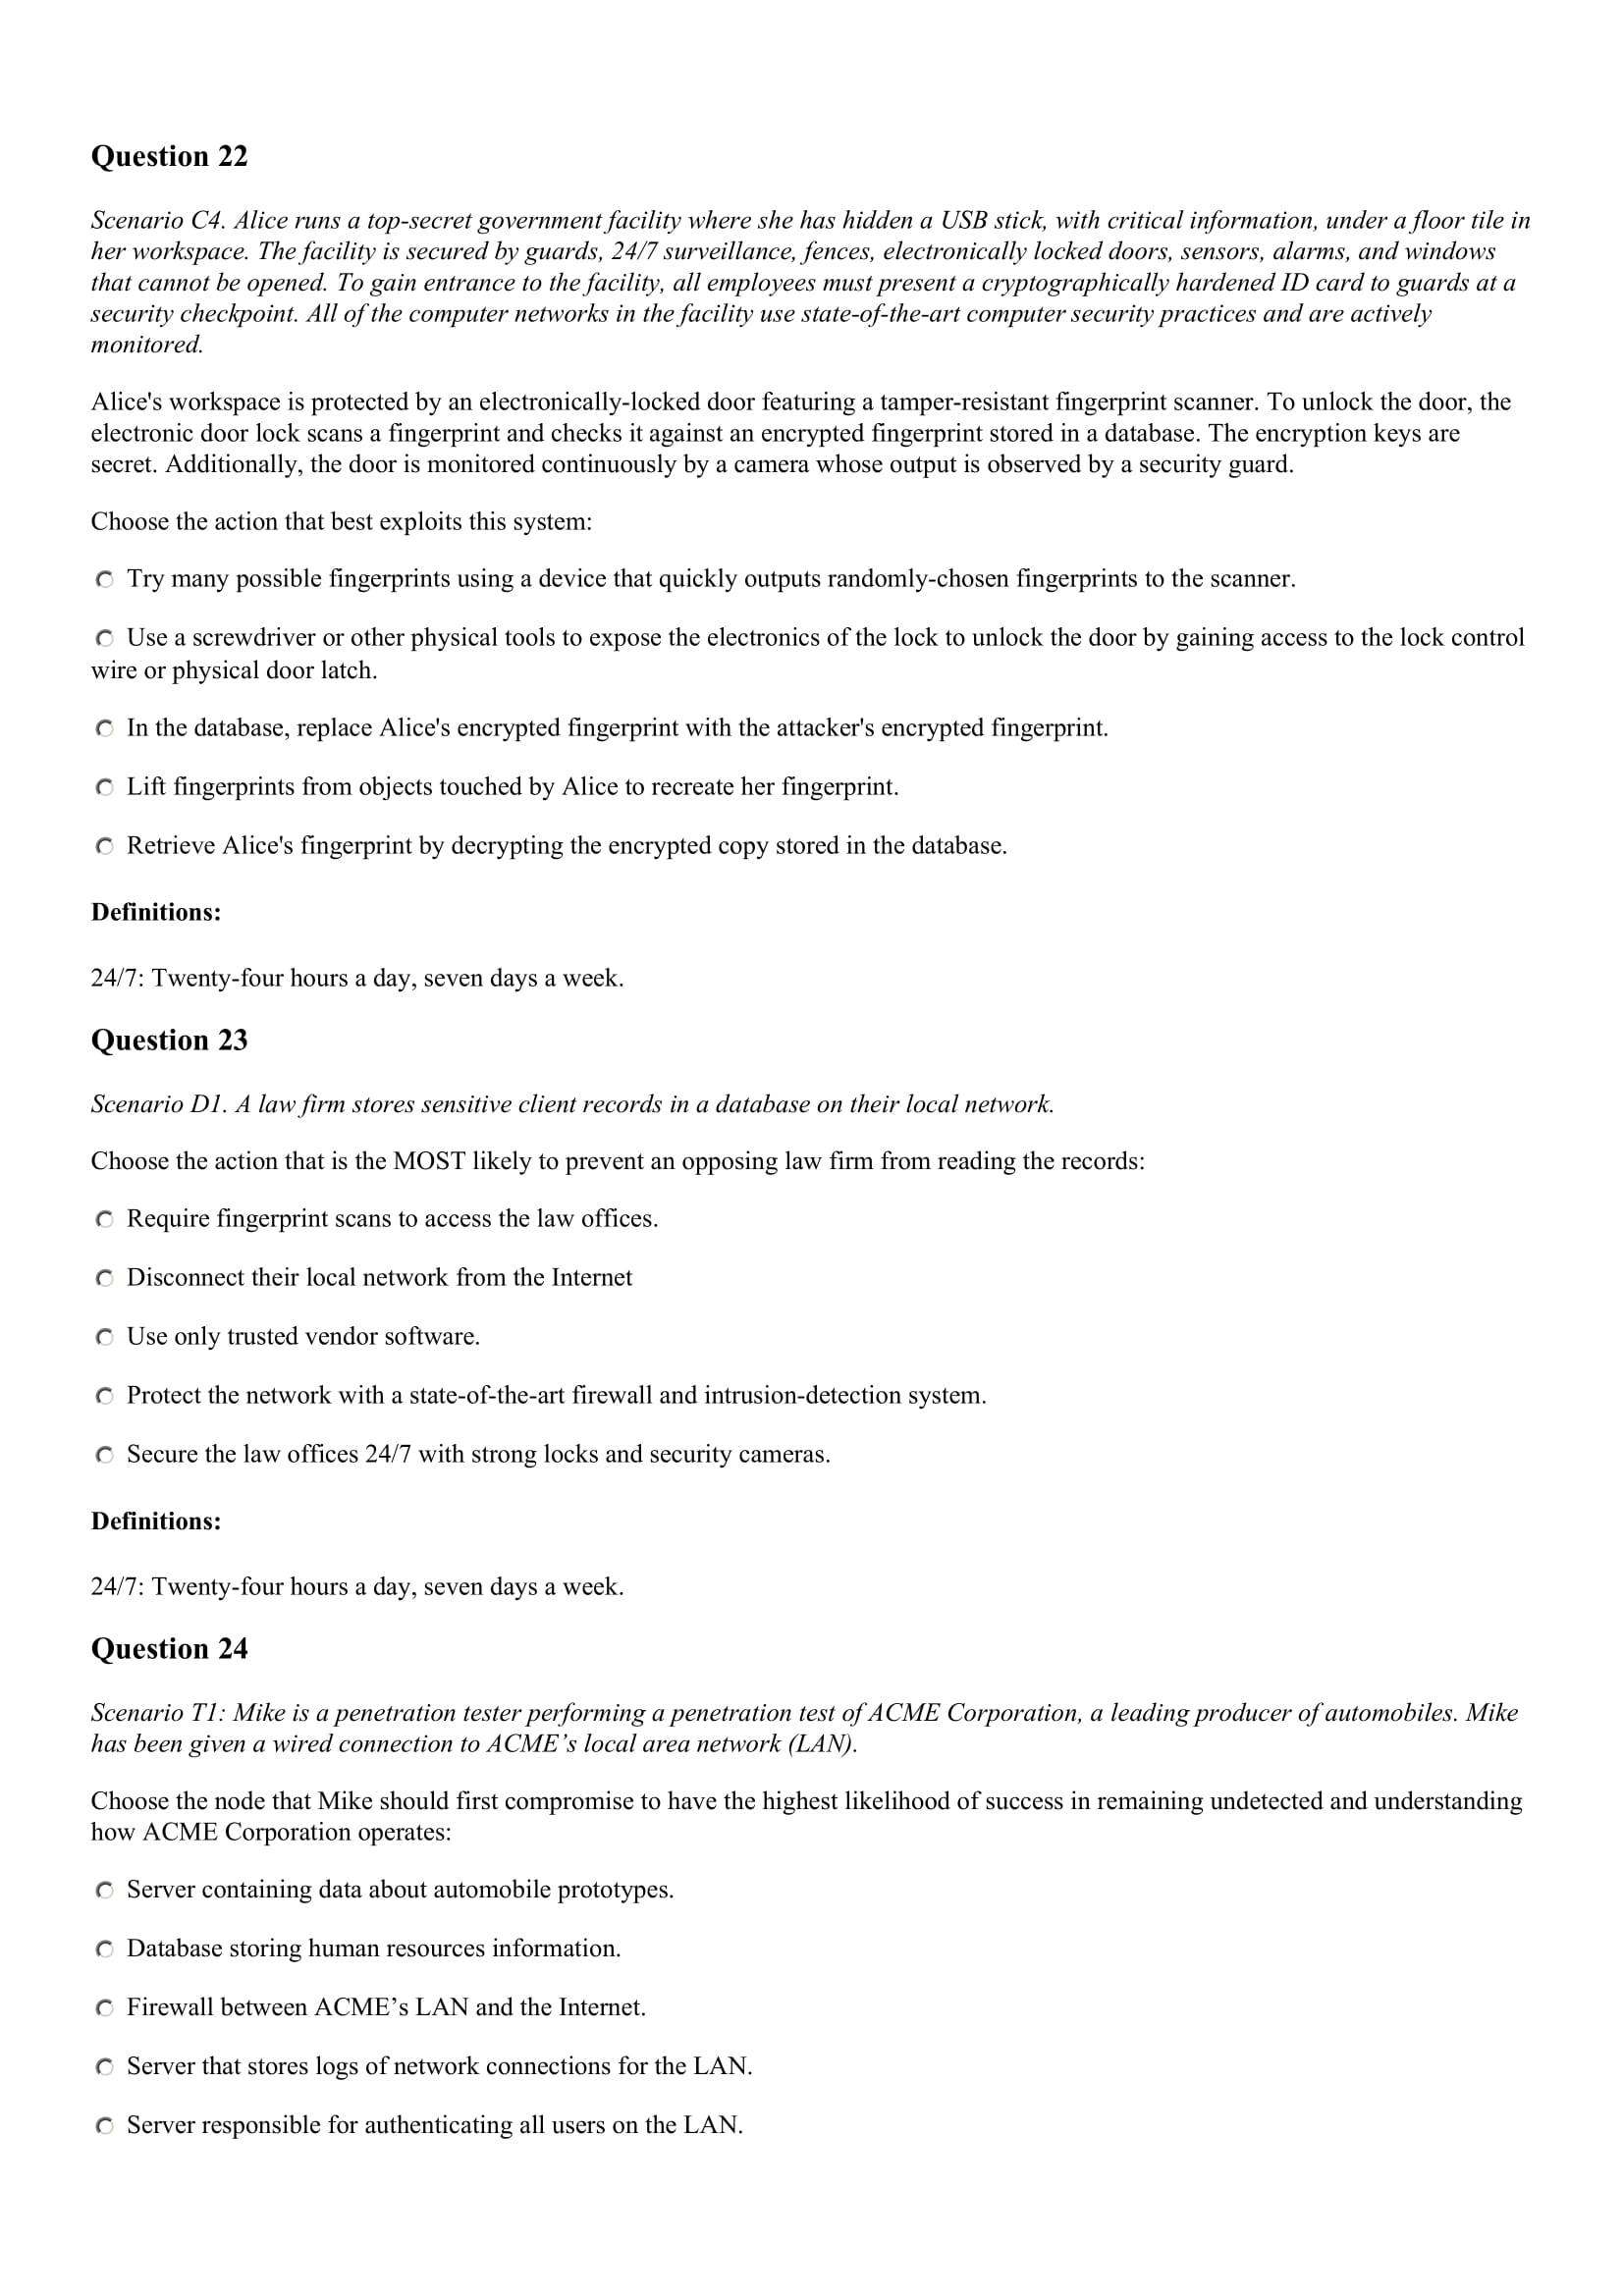
\includegraphics[scale=.25]{images/exam/correctly_formated_exam-10.jpg}
    \label{fig:correctly_formated_exam-10}
\end{center}
\end{figure}

\begin{figure}[!h]
    \begin{center}
    \advance\leftskip-3cm
    \advance\rightskip-3cm
    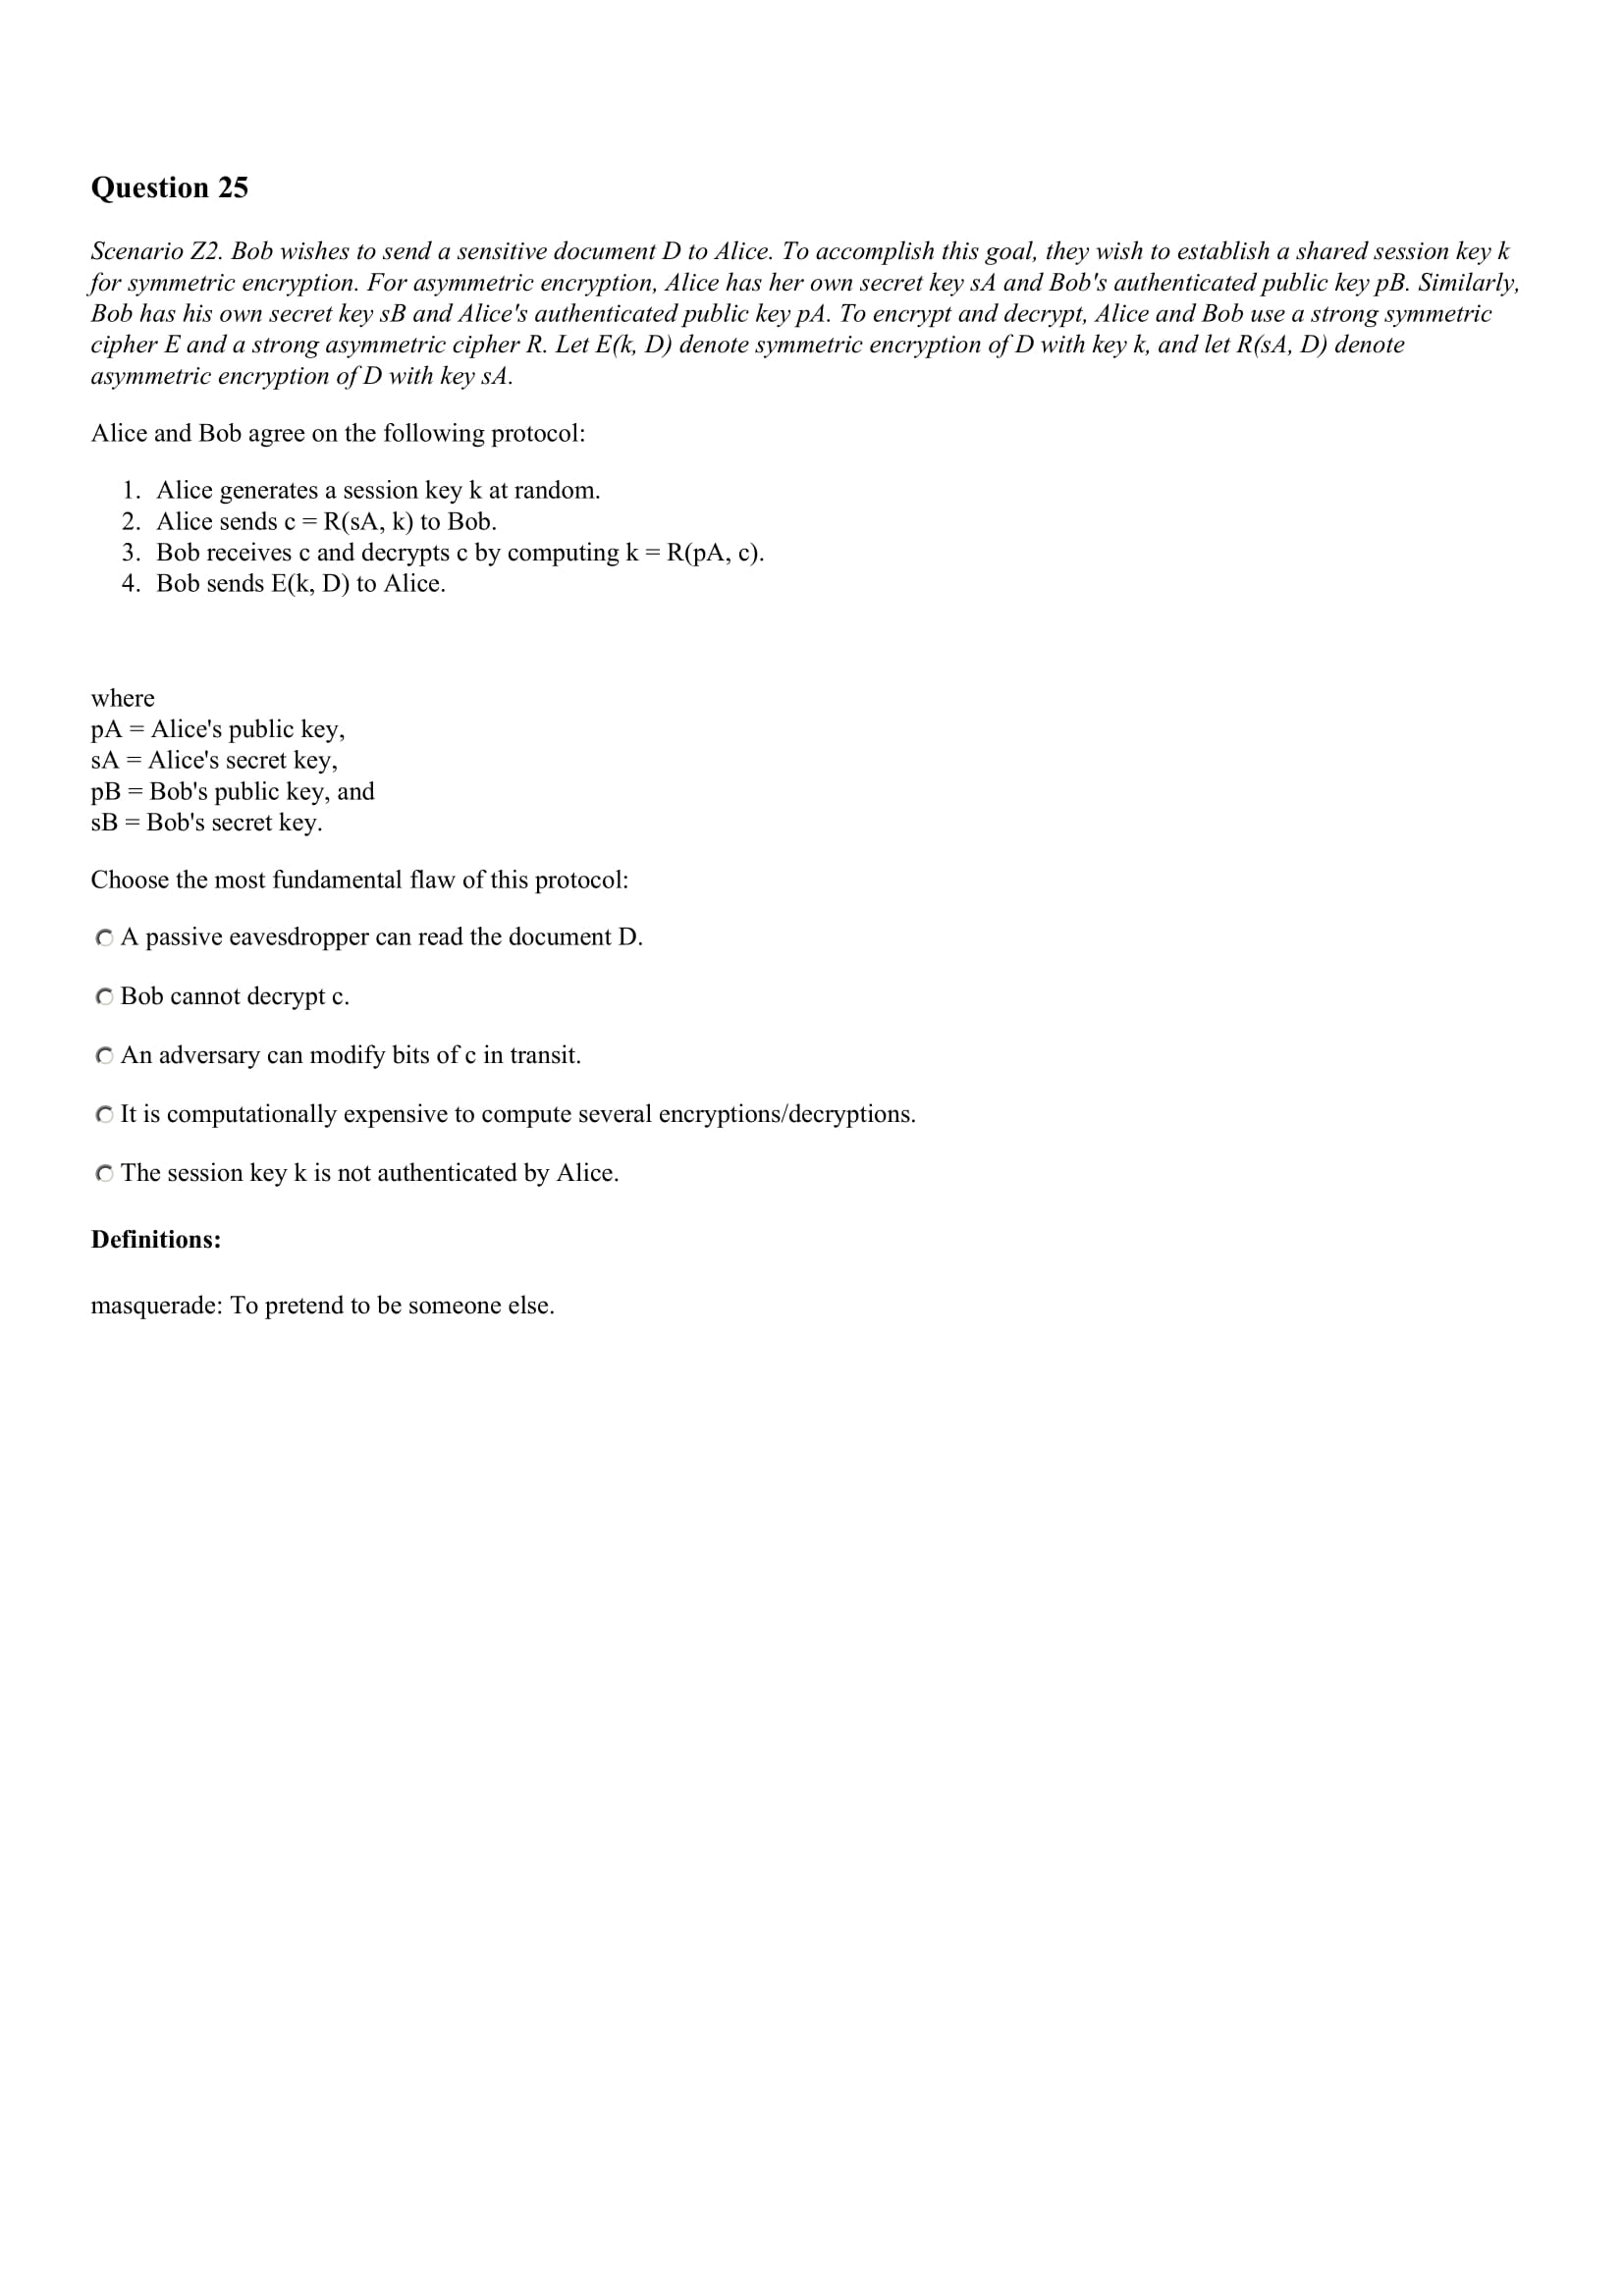
\includegraphics[scale=.25]{images/exam/correctly_formated_exam-11.jpg}
    \label{fig:correctly_formated_exam-11}
\end{center}
\end{figure}

%%%%%%%%%%%%%%%%%%%%%%%%%%%%%%%%%%%%%%%%%%%%%%%%%%%%%%%%%%%%%%%%%%%%%%%%%%%%%%%
% AUTHOR'S BIOGRAPHY
% As of 10/03/2011, Author's Biography or Vita no longer accepted by Grad College

\end{document}
\endinput
